\documentclass[12pt]{report}
\usepackage[latin1]{inputenc} 
\usepackage[T1]{fontenc}
\usepackage[english, francais]{babel}
\usepackage{dsfont}
\usepackage{framed}
\usepackage{listings}


\usepackage[top=3cm, bottom=3.5cm, left=3cm, right=3cm]{geometry}
\usepackage[colorlinks=true]{hyperref}
\title{Dyson brownian motion and statistical applications}
\author{S�bastien \bsc{Ohleyer}}

%%% Section's headings indent %%%
\usepackage{titlesec}
	\titleformat{\section}[block]{\bf\Large}{\thesection.}{1em}{} 
	\titleformat{\subsection}[block]{\hspace{2em}\bf\large}{\thesubsection}{1em}{}
	% \titleformat{\subsubsection}[block]{\hspace{4em}\bf\large}{\thesubsubsection}{1em}{}

%%% Name of the Bibliographe page
\renewcommand{\bibname}{References}
\usepackage[backend=biber, style=alphabetic, sorting=nyt]{biblatex}
\addbibresource{biblio.bib}

%%% Maths packages setup %%%
\usepackage{amsfonts,amssymb,dsfont,amsmath,mathtools,amsthm,stmaryrd,bm,array}
	\newtheoremstyle{break}{.3cm}{.3cm}{\itshape}{}{\bfseries}{}{\newline}{}
	\theoremstyle{break} 
	\newtheorem{theorem}{Theorem}[section]
	\newtheorem{lemma}[theorem]{Lemma}
	\newtheorem{proposition}[theorem]{Proposition}
	\newtheorem{definition}[theorem]{Definition}
	\newtheoremstyle{break_rem}{.3cm}{.3cm}{}{}{\it}{}{\newline}{}
	\theoremstyle{break_rem}
	\newtheorem{remark}[theorem]{Remark}
	\newtheorem{corollary}[theorem]{Corollary}
\usepackage{algorithm,algorithmic,eqparbox}
\renewcommand\algorithmiccomment[1]{\hfill\#\ \eqparbox{COMMENT}{#1}}

%%% Images and figures
\usepackage{tikz,caption}
\usepackage{graphicx}


\begin{document}
\selectlanguage{english}
	
\newpage
\strut
\newpage
\tableofcontents
\newpage
%\strut
%\newpage
\chapter*{Acknowledgements}
	\addcontentsline{toc}{chapter}{Acknowledgements}
	I would like to warmly thank my two supervisors Myl�ne Ma�da and R�mi Bardenet. They believed in me and entrusted this particularly interesting subject for my master's thesis. During all of the year, they have supported me and have spent so much time helping me and teaching some new mathematical concepts. For all of this, I am extremely grateful to them.\\

	It was a real pleasure to work with them on this subject. I was intensely interested in every part of the topic, which was finally very diverse. In the future, I would sincerely like to carry out other projects related to it.\\

	Finally, I also thank Andr� de Laire and Pierre Chainais - respectively in the name of the Universit� de Lille and the Ecole Centrale de Lille - for making this master's thesis work possible by a collaboration between the schools. It was a great experience for me to discover the world of research and would like to stay close to it during the next years. I strongly think that an engineer needs to achieve research projects like this and understand state-of-the-art research papers to continuously develop his scientific knowledge.

\chapter*{Introduction}
	\addcontentsline{toc}{chapter}{Introduction}
		The eigenvalues of some specific random matrices - e.g. Gaussian Unitary Ensemble matrices (GUE) - have distinctive properties, especially when we consider them as a collection of points. We can note a special interaction between the eigenvalues, characterised by a \textit{repulsion}, and show that the set of eigenvalues form a \textit{determinantal point process} (DPP). Moreover, random matrix can be propagate over time regarding a matrix-valued random process as a solution of a matrix-valued \textit{Stochastic Differential Equation} (SDE). Going further, we can link these two ideas and consider the eigenvalues processes of a matrix-valued random process. Eigenvalues processes are solutions of scalars SDEs and define some trajectories over time. In practise, the eigenvalues trajectories also display a significant repulsion. \\

		The Dyson Brownian motion \cite{dyson1962brownian} describes the evolution of the eigenvalues of a matrix-valued random process, the Hermitian Brownian motion. It defines a system of scalar SDEs verified by the eigenvalues, generating eigenvalues trajectories that exactly highlight an interesting repulsion. In addition, the value of the Hermitian Brownian motion at a $t=1$ is a GUE matrix, hence its eigenvalues collection form a DPP. Here, we see the point of our work, we want to understand the link between the static repulsion in a set of eigenvalues and the dynamic repulsion in eigenvalues trajectories. We can study this connection from two points of view : the random matrix SDE and the system of SDEs satisfyed by the associated eigenvalues, which give different simulation methods with their pros and cons.\\ 

		We will try to give a justification of the dynamic repulsion and an explaination of the nature of this repulsion, keeping in mind the simulation issue.
		A complete overview of the most classical example - the Dyson Brownian motion - is provided in Chapter \ref{ref : chap 1 DBM} (mostly referring to \cite{agz}). Furthermore, we present two other examples, to spotlight the variety of these processes. Then in Chapter \ref{chap 2}, we will focus on the link between a SDE satisfyed by a matrix-valued random process and the system of SDEs verifyed by the associated eigenvalues processes (based on \cite{taotopics,grac}). Finally, we will examine two very recent papers \cite{dumitriu2002matrix,2017arXiv170702700H} in Chapter \ref{chap3}. They propose a new approach to this problem considering tridiagonal models, which can be clever way to deal with simulations.

%\newpage
%\strut
%\newpage

\chapter{The Dyson Brownian motion and other classical processes}\label{ref : chap 1 DBM}
	In this study, we are interested in the link between the matrix-valued random process and the eigenvalues processes, and on its ability to reflect a repulsion. Before focusing on this link, we will deal with the most classical example of this type of processes, the Dyson Brownian motion \cite{dyson1962brownian} . The objects manipulated in this study are complex and it is hard to link them in a general way.  \newline

	However, it seemed to be essential to expose at least one complete example presenting those three different aspects. This first part will introduce the Dyson Brownian motion, which is the simplest illustration of the relations we want to expose here. \newline
	We will start by introducing some results for the static case, meaning that we only consider a random matrix and not a matrix-valued random process yet. Then, we will expose the general example of the Dyson Brownian motion and finally some other well-known examples.

	\section{Static random matrices and eigenvalues} % (fold)
	\label{sec:static_random_matrices_and_eigenvalues}
		We start by defining some useful matrices for this study (Section \ref{sub:random_matrices}), and classical results about their eigenvalues (Section \ref{sub:eigenvalues_of_random_matrices}). Finally, Section \ref{sub:determinantal_point_process} gives a brief introduction to determinantal point processes (sometimes written as DPP) and to the link between GUE eigenvalues and this type of point processes.

		\subsection{Random matrices} % (fold)
		\label{sub:random_matrices}
			Let $\mathcal{N}_{\mathbb{R}}(0,1)$ denotes the real standard normal distribution and $\mathcal{N}_{\mathbb{C}}(0,1)$ the complex standard normal distribution. Note that $Z \sim \mathcal{N}_{\mathbb{C}}(0,1)$ if$\ Z=(R+\mathrm{i}S)/\sqrt{2}$ with$\ R$ and$\ S$ independent and $R,S \sim \mathcal{N}_{\mathbb{R}}(0,1)$.\\ 
			We recall the definition of Ginibre matrices and Gaussian Unitary Ensemble (GUE) matrices.
			
			\begin{definition}[Ginibre matrices]\label{gin-mat-def}
				Considering a$\ N\times N$ matrix $M$ with independent entries$\ (M_{ij})_{1\leq i,j\leq N}$, $M$ is a Ginibre matrix if$\ M_{ij} \sim \mathcal{N}_{\mathbb{C}}(0,1/N)$ for $1\leq i,j\leq N$.
			\end{definition}
			Using Ginibre matrices, we can define the Gaussian Unitary Ensemble (GUE).
			\begin{definition}[Gaussian Unitary Ensemble (GUE) matrices]\label{gue-mat-def}
				Let $M$ be a $N\times N$ Ginibre matrix, we define $G$ as follows : \[ G = \frac{M+M^*}{\sqrt{2}} \]
				with $M^* = \overline{M}^T$ the conjugate transpose of $M$. Then, $G$ is a \emph{GUE(N)} matrix.
			\end{definition}

			\begin{remark}\label{rem : gue def}
					GUE matrices can also be described as Hermitian matrices (i.e. $G^*=G$) where the diagonal entries are i.i.d. random variables following the distribution$\ \mathcal{N}_{\mathbb{R}}(0,1/N)$ and the upper-triangular entries are i.i.d. with distribution$\ \mathcal{N}_{\mathbb{C}}(0,1/N)$.\\ 
					Indeed, for $j=i$
					\begin{equation}
						Var(G_{ii})=\mathbb{E}[G_{ii}^2]=\mathbb{E}\left[\left(\frac{M_{ii}+\overline{M_{ii}}}{\sqrt{2}}\right)^2\right]=\mathbb{E}[R_{ii}^2]=Var(R_{ii})=1/N \notag
					\end{equation}
					and for $j>i$
					\begin{align}
						Var(G_{ij})=\mathbb{E}[|G_{ij}|^2]=\mathbb{E}\left[\left|\frac{M_{ij}+\overline{M_{ji}}}{\sqrt{2}}\right|^2\right]&=\mathbb{E}\left[\left|\frac{R_{ij}+R_{ji}+\mathrm{i}(S_{ij}-S_{ji})}{2}\right|^2\right] \notag \\
						&= \mathbb{E}\left[\frac{(R_{ij}+R_{ji})^2+(S_{ij}-S_{ji})^2}{4}\right] \notag\\
						&=\frac{1}{4}(Var(R_{ij}+R_{ji})+Var(S_{ij}-S_{ji}))\notag \\
						&=1/N \notag
					\end{align}
					GUE matrices have the following density with respect the Lebesgue measure on the Hermitian matrices space
					\begin{align}\label{eq : GUE distribution}
						d\mathbb{P}(G)&=\prod_{i=1}^N\sqrt{\frac{N}{2\pi}}\exp\left({\frac{-Ng_{ii}^2}{2}}\right)\prod_{1\leq i<j\leq N}\frac{N}{\pi}\exp\left({-N|g_{ij}|^2}\right) \notag \\
						&=\left(\frac{N}{2\pi}\right)^{N/2}\left(\frac{N}{\pi}\right)^{N(N-1)/2}\exp\left(-\frac{N}{2}\left(\sum_{i=1}^Ng_{ii}^2+2\sum_{1\leq i<j\leq N}|g_{ij}|^2\right)\right) \notag \\
						&=\frac{1}{2^{N/2}}\left(\frac{N}{\pi}\right)^{N^2/2} \exp\left(-\frac{N}{2}Tr(G^2)\right)
					\end{align}
			\end{remark}

			After this introduction of the fundamental matrix ensemble used further in this study - the GUE - we give some results about their eigenvalues. In fact, some precise results exist on their distribution in a static framework and one idea of our analysis is to see if these results are still available in a dynamic framework.
		% subsection random_matrices (end)

	% section static_random_matrices_and_eigenvalues (end)

		\subsection{Eigenvalues of random matrices} % (fold)
		\label{sub:eigenvalues_of_random_matrices}
			In this part, we aim to give fundamental results about GUE eigenvalues. The first result concerns the eigenvalues \textit{empirical distribution}.\newline
			If we naively represent the histogram of eigenvalues of a GUE matrix, we can see on Figure \ref{fig : dpp_gue_rescale} that a particular type of distribution appears.
			\begin{figure}[h] \centering
					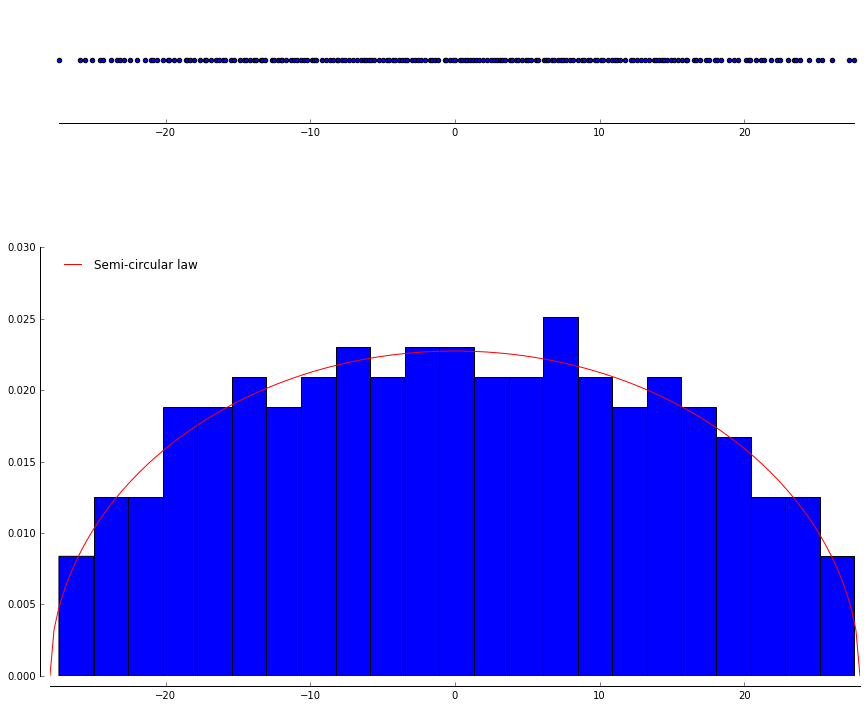
\includegraphics[width=.6\textwidth]{images/gue_eigenvalues.png}
				    \caption{\textbf{Eigenvalues histogram of a GUE matrix}, generated by GUE(200) matrix diagonalisation.}\label{fig : dpp_gue_rescale}
			\end{figure} \newline
			Now, let us explain mathematically this phenomenon. We denote by $\ (\lambda_i)_{1\leq i\leq N}$ the (real) eigenvalues of a GUE matrix, ordered such that$\ \lambda_1<\lambda_2<...<\lambda_N$. Note that because $(\lambda_i)_{1\leq i\leq N}$ are eigenvalues of a GUE matrix, they are almost surely distincts. We define the empirical distribution of the eigenvalues as the probability measure on$\ \mathbb{R}$
			\begin{equation}\label{eq : empirical distribution}
				\widehat{\mu}_N=\frac{1}{N}\sum_{i=1}^N \delta_{\lambda_i}
			\end{equation}

			We also define the \textit{semicircle distribution} as the probability distribution$\ \sigma(x)dx$ on$\ \mathbb{R}$ with density
			\begin{equation}\label{eq : semicircle distribution}
				\sigma(x)=\frac{1}{2\pi}\sqrt{4-x^2}\mathds{1}_{|x|\leq2},
			\end{equation}\newline
			Then we can present the Wigner theorem in the particular case of GUE matrices. Note that Theorem \ref{th : wigner} has been proved for more general matrices than GUE matrices in \cite{Wig55,agz}. For this theorem, let us define a sequence of GUE matrices $(G_N)_{N>0}$ with growing dimensions: $G_1\sim$ GUE(1), $G_2\sim$ GUE(2) until $G_N\sim$ GUE(N). On this sequence of matrices, we define the sequence of eigenvalues empirical distributions $(\widehat\mu_N)_{N>0}$ of these matrices.

			\begin{theorem}[Wigner Theorem]\label{th : wigner}
				For a sequence $(G_N)_{N>0}$ of \emph{GUE} matrices (as previously defined), the sequence of empirical measures $(\widehat\mu_N)_{N>0}$ converges weakly, in probability, to the semicircle distribution.
			\end{theorem}

			Another well-known aspect of the GUE eigenvalues is their joint distribution. The following result was given in \cite{agz}.
			
			\begin{theorem}[Joint distribution of GUE eigenvalues]\label{th : joint distrib GUE}
				Let $G$ be a \emph{GUE(N)} matrix, the joint distribution of the eigenvalues$\ \lambda_1<\lambda_2<...<\lambda_N$ has density with respect to the Lebesgue measure which equals 
				\begin{equation}\label{eq : gue join distrib}
					u_N(x_1,...,x_N)=C_N\Delta_N(x)^2\prod_{i=1}^Ne^{-Nx_i^2/2}\mathds{1}_{\{x_1<x_2<\dots<x_N\}}
				\end{equation}
				where
				\begin{align}
					C_N&=N!\left(\int_{-\infty}^{\infty}...\int_{-\infty}^{\infty}\Delta_N(x)^2\prod_{i=1}^Ne^{-Nx_i^2/2}dx_i\right)^{-1} \notag\\
					&=\left(\frac{N^N}{2\pi}\right)^{N/2}\frac{1}{\prod_{j=1}^N(j-1)!}
				\end{align}
				and $\ \Delta_N(x) = \prod_{1\leq i<j\leq N}(x_i-x_j)$ is the Vandermonde determinant.
			\end{theorem}
			Having the joint distribution of the eigenvalues, we can go further and see the set of GUE eigenvalues on a different point of view. Indeed, the collection of eigenvalues of a GUE matrix can be considered as a configuration of points on $\mathbb R$, namely a \textit{point process}. Let us introduce the very basics of this kind of processes in the next section.
		% subsection eigenvalues_of_random_matrices (end)


		\subsection{Determinantal point processes} % (fold)
		\label{sub:determinantal_point_process}
			In this study, we introduce very briefly real determinantal point processes. For a more general study, the reader could refer to \cite{agz}, Section 4.2. Let us start by defining configuration of points before exposing the definition of a point process.
			\begin{definition}[Configuration (of points)]\label{def : configuration de points}
				A configuration of points $\gamma$ is a subset of $\mathbb R$, dicrete and locally finite :
				\begin{itemize}
					\item Discrete : $\forall x\in \gamma, \exists r>0, \hspace{0.5cm} B(x,r)\cap\gamma=\{x\}$
					\item Locally finite : $\forall K \subset \mathbb R$,\ K compact,\hspace{0.5cm} $\#(\gamma\cap K)<\infty$
				\end{itemize}
			\end{definition}
			\begin{definition}[Point process (simple)]\label{def : point process simple}
				A point process is a random configuration of points $\gamma$. By random, we mean that it exists a probability measure on the set of configurations, equipped with a standard $\sigma$-algebra, which make $\gamma\rightarrow\#(\gamma\cap K)$ mesurable for all compact K.
			\end{definition}
			From now, let us note $\mu$ the reference measure on $\mathbb R$. Determinantal point processes have their name because of the particular form of their \textit{joint intensities}.

			\begin{definition}[Joint intensities]\label{def : correlation functions}
				Considering a point process defined with respect to $\mu$, for all $k\geq1$, its $k$-correlation function is defined by
				\[\mathbb{E}\left[\sum_{\substack{(X_1,\dots,X_k) \\ X_1 \neq \dots \neq X_k \in \gamma}}f(X_1,\dots,X_k) \right]
                = \int_{\mathbb X^k} f(x_1,\dots,x_k) \rho_k(x_1,\dots,x_k) \mu(dx_1) \cdots \mu(dx_k) \]
                for all $f :\mathbb R^k\rightarrow \mathbb C$ mesurable with compact support.
			\end{definition}
			Then, we can introduce a particular type of point processes, the \textit{determinantal point processes}.
			\begin{definition}
				A point process on $\mathbb R$ with respect to $\mu$ is determinantal if kernel $K:\mathbb R\times\mathbb R\rightarrow\mathbb C$ exists so that 
				\[\rho_k(x_1,...,x_k)=\det[K(x_i,x_j)]_{1\leq i,j\leq k}\]
				for all $k\geq1$ and $x_1,...,x_k\in\mathbb R$.
			\end{definition}
			As the last definition shows, the singularity of determinantal point processes is to have their joint intensities which can be written as a determinant of a matrix, namely the \textit{kernel}.\\
			Let us momentarily set $N=2$ and consider a collection of 2 random variables, in order to understand the influence of the kernel. We compute some classical probability densities.\\
			The joint density of $(X_1,X_2)$ is
		            \begin{equation*}
		                f_2(x,y) = \frac12 \left(K(x,x)K(y,y) - |K(x,y)|^2 \right)
		            \end{equation*}
		    to compute the marginal density, we integrate with respect to one of the variable and get
		            \begin{equation*}
		                f_1(x) = \frac12 K(x,x)
		            \end{equation*}
		    The conditional density of $X_2 | X_1$ is then given by
		            \begin{equation*}
		                f_{2|1}(y) 
		                = \frac{f_2(X_1,y)}{f_1(X_1)}
		                = K(y,y) - \frac{|K(X_1,y)|^2}{K(X_1,X_1)}
		            \end{equation*}
		    In this last formula, we notice the \textit{repulsion} between the two random variables. Indeed, the more $y$ is close to $X_1$ (i.e. $y$ and $X_1$ are highly correlated), the more the conditional density is small.\\
		    
			Getting back to GUE matrices, the collection of their eigenvalues can actually be viewed as a determinantal point process with a particular kernel. The following theorem expose this result.

			\begin{theorem}[Kernel of the DPP generated by the eigenvalues of a GUE matrix]\label{th : kernel eig GUE}
				Considering a \emph{GUE(N)} matrix, the collection of its eigenvalues $\{\lambda_1,...,\lambda_N\}$ is a determinantal point process with a kernel $K_N$ defined by
				\begin{equation}\label{eq : kernel GUE}
					K_N(x,y)=\sum_{i=0}^{N-1}\frac{h_i(x)h_i(x)}{||h_i||^2}e^{-N(x^2+y^2)/4} 
				\end{equation}
				with $(h_i)_{0\leq i\leq N-1}$ the orthogonal polynomial with respect to the measure $e^{-Nx^2/2}dx$ and with leading coefficient 1 (a.k.a the Hermite polynomials).
			\end{theorem}

			This result is not straightforward and we usually employ the following theorem, presented in \cite{Joh06}, to prove it.

			\begin{theorem}\label{th : joh criteria}
				Let us consider$\ (\phi_i)_{1\leq i\leq N}$ and$\ (\psi_j)_{1\leq j\leq N}$ be measurable functions such as $\phi_i\psi_j$ is integrable for any$\ i,j$. Supposing that the random vector $(X_1,...,X_N)\in\mathbb{R}^N$ has a density with respect to the reference measure :
				\begin{equation}
					u_N(x_1,...,x_N)=\frac{1}{Z_NN!}\det[\phi_i(x_j)]_{i,j=1}^N\det[\psi_i(x_j)]_{i,j=1}^N
				\end{equation}
				where 
				\begin{equation}
					Z_N=\frac{1}{N!}\int_{\mathbb{X}^N}\det[\phi_i(x_j)]_{i,j=1}^N\det[\psi_i(x_j)]_{i,j=1}^N\mu^{\otimes N}(dx)
				\end{equation}
				Then, the associated point process$\ \{X_1,...,X_N\}$ is determinantal and its kernel is given by :
				\begin{equation}\label{eq : general_kernel}
					K_N(x,y)=\sum_{i,j=1}^N\phi_i(x)[A^{-1}]_{ij}\psi_j(x)
				\end{equation}
				where$\ A$ is a$\ N\times N$ matrix with entries
				\begin{equation}
					A_{ij}=\int_{\mathbb{X}}\psi_i(x)\phi_j(x)\mu(dx)
				\end{equation}
			\end{theorem}

			\begin{proof}[Proof of \ref{th : joh criteria}]
				We do not detail the proof here but the reader could refer to \cite{Joh06}.
			\end{proof}

			\begin{proof}[Proof of \ref{th : kernel eig GUE}]
			Now, we aim to apply Theorem \ref{th : joh criteria} to Equation \eqref{eq : gue join distrib}. Forgetting about the normalisation factor$\ C_N$, we have
			\begin{align}\label{eq : determinant row operation}
				\Delta_N(x)^2\prod_{i=1}^Ne^{-Nx_i^2/2} = \left(\det[x_i^{j-1}]_{i,j=1}^N\right)^2\prod_{i=1}^Ne^{-Nx_i^2/2} &= \left(\det[x_i^{j-1}e^{-Nx_i^2/4}]_{i,j=1}^N\right)^2 \notag \\
				& = \left(\det[x_j^{i-1}e^{-Nx_j^2/4}]_{i,j=1}^N\right)^2
			\end{align}
			
			We can now set
			\begin{equation}
				\phi_i(x)=\psi_i(x)=x^{i-1}e^{-Nx^2/4}
			\end{equation}
			So that
			\begin{equation}
				A_{ij}=\int_{\mathbb{R}}\phi_i(x)\psi_i(x)dx = \int_{\mathbb{R}}x^{i+j-2}e^{-Nx^2/2}dx \notag
			\end{equation}
			With these choices of $\phi_i$ and $\psi_i$, the matrix $A$ can be tough to inverse. Recall that these choices are motivated by the value of the determinant in Equation \eqref{eq : determinant row operation}, the classical property of the determinant allow us to do row operations - like linear combinations - without changing its value. Hence, we have
			\begin{equation}
				\det[x_j^{i-1}e^{-Nx_j^2/4}]_{i,j=1}^N = \det[h_{i-1}(x)e^{-Nx_j^2/4}]_{i,j=1}^N  
			\end{equation}
			with $(h_i)_{0\leq i\leq N-1}$ an arbitrary sequence of polynomials of degree $i-1$ and leading coefficient 1.
			Thus, by chosing for $(h_i)_{0\leq i\leq N-1}$ the orthogonal polynomial with respect to the measure $e^{-Nx^2/2}dx$ and with leading coefficient 1, we set
			\begin{equation}
				\phi_i(x)=\psi_i(x)=h_{i-1}(x)e^{-Nx^2/4} \notag
			\end{equation}
			and the entries of matrix$\ A$ become
			\begin{equation}
				A_{ij}=\int_{\mathbb{R}}\phi_i(x)\psi_i(x)dx = \int_{\mathbb{R}}h_{i-1}(x)h_{j-1}(x)e^{-Nx^2/2}dx=||h_{i-1}||^2\delta_{ij} \notag
			\end{equation}
			where$\ ||h_i||^2=\int_{\mathbb{R}}h_i(x)^2e^{-Nx^2/2}dx$. $A$ becomes a diagonal matrix and is now easy to inverse. \\
			According to the general expression of the kernel \eqref{eq : general_kernel}, we do not need to care about the normalisation factor $C_N$. Indeed, if we decide to separate it in two and put it in the expression of$\ \phi_i$ and$\ \psi_i$, it will be balanced by the expression of$\ [A^{-1}]_{ij}$.\\

			We can now apply Theorem \ref{th : joh criteria} and write the kernel$\ K_N$ of the point process$\ \{\lambda_1,...,\lambda_N\}$
			\begin{equation}
				K_N(x,y)=\sum_{i=0}^{N-1}\frac{h_i(x)h_i(y)}{||h_i||^2}e^{-N(x^2+y^2)/4} \notag
			\end{equation}
			\end{proof}
			Regarding that GUE eigenvalues are determinantal processes, they also have the particular repulsion property. Our idea is to understand how this property can be spread dynamically. For this purpose, we will now present the Dyson Brownian motion. From now, we will exposed some processes varying over time. They will also be called processes but they are very different from point processes in nature (Definition \ref{def : point process simple}). Scalar-valued processes and matrix-valued processes refer to processes varying with time while determinantal point processes indicate point process at a fixed time. 

		% subsection determinantal_point_process (end)

	\section{The Dyson Brownian motion} % (fold)
	\label{sec:the_dyson_brownian_motion}
		Before exhibiting the Dyson Brownian motion, we need to introduce some notations in Section \ref{sub:notation} and to motivate our analysis in Section \ref{sub:Random matrix-valued process} and \ref{sub:eigenvalues joint distribution over time}. Section \ref{sub:eigenvalues joint distribution over time} also links the dynamic framework to the static one, concerning the eigenvalues joint distribution and we finally present the Dyson Brownian motion in Section \ref{subsection : DBM matrix - ev}.
		\subsection{Notation} % (fold)
		\label{sub:notation}
			In the following study, we deal with several different mathematical objects, that is why it seems important to directly clarify the notation for these objects. We will use the same notation as in \cite{2017arXiv170702700H}. Matrix-valued processes $\pmb X=(X_t)_{t\geq 0}$ will be noted in bold whereas $X_t$ denote the value of the process $\pmb X$ at a fixed time $t$. Then $\pmb X_{ij}$ refers to the scalar-valued process of the entry $(i,j)$ of $\pmb X$ and the value of $\pmb X_{ij}$ at the time $t$ will be denoted $X_{ij,t}$.\\
			Concerning the eigenvalues processes of a matrix process, we consider them ordered. In most cases, they will be strictly ordered except for the initial conditions. For example, if there are $N$ processes, we order them so that $\lambda_1(t)<\lambda_2(t)<...<\lambda_{N-1}(t)<\lambda_N(t)$ for $t>0$ and $\lambda_1(0)\leq\lambda_2(0)\leq...\leq\lambda_{N-1}(0)\leq\lambda_N(0)$. The $i$th eigenvalue process $(\lambda_i(t))_{t\geq0}$ of the matrix-valued process will be noted $\lambda_i(t)$. \\
			Moreover, if we consider a simple scalar-valued random process which is not an entry of a matrix neither an eigenvalue of a matrix, we will denote it simply $(Z(t))_{t\geq0}$.
		% subsection notation (end)

		\subsection{Random matrix-valued process and its eigenvalues processes} % (fold)
		\label{sub:Random matrix-valued process}
			Now, we introduce the Hermitian Brownian motion (as in \cite{agz}) which is the very classical matrix-valued process and the starting point of this study.

			\begin{definition}[Hermitian Brownian motion]\label{herm-mat-def}
				Let$\ (\pmb B_{kl}^1)_{1\leq k\leq l\leq N}$ and$\ (\pmb B_{kl}^2)_{1\leq k<l\leq N}$ be two independent collections of i.i.d. real valued standard Brownian motions. The Hermitian Brownian motion denoted $\pmb H$ is the random process with entries $(\pmb H_{kl})_{1\leq k,l\leq N}$ so that 
				\begin{align*}
					\pmb H_{kl}= \left\{
			    					\begin{array}{ll}
			        					\frac{1}{\sqrt{2N}}(\pmb B_{kl}^1+\mathrm{i}\pmb B_{kl}^2) & \emph{if}\ k<l  \\
			        					\frac{1}{\sqrt{2N}}(\pmb B_{lk}^1-\mathrm{i}\pmb B_{lk}^2) & \emph{if}\ k>l  \\
			        					\frac{1}{\sqrt{N}}\pmb B_{kk}^1 & \emph{if}\ k=l
			    					\end{array}
								\right.
				\end{align*}
			\end{definition} \vspace{0.5cm}

			With this definition, we can deduce an exact way of simulating such kind of process. Indeed, using the independence and the law of the Brownian motion's increments, we can explain the following theorem, useful for the simulations.

			\begin{lemma}\label{th : HBM increments}
				Let $\pmb H$ be a $N\times N$ Hermitian Brownian motion. The increments of $\pmb H$ are independent and follow the law $H_t-H_s\sim\sqrt{t-s}\ G$ with $G\sim$ \emph{GUE(N)}.
			\end{lemma}

			Assuming that we have a random matrix SDE satisfied by a$\ N\times N$ matrix process $\pmb X$, for example :$\ X_t=A+H_t$ with $A$ a$\ N\times N$ Hermitian matrix and $\pmb H$ a$\ N\times N$ Hermitian Brownian motion as defined in \ref{herm-mat-def}.
			\begin{remark}[First definition of a matrix SDE]\label{rem: SDE first def}
				At this point of the study, let us assume that a SDE is define by an equation like $X_t=A+H_t$, where $A$ is an initial condition and $\pmb H$ a$\ N\times N$ Hermitian Brownian motion. SDE will be define in a more general way, for scalars and matrices in Section \ref{subsect : O-U process intro}.
			\end{remark}

			Lemma \ref{th : HBM increments} provides a way to \textbf{exactly simulate} eigenvalues trajectories of $\pmb X$, using the random matrix SDE, as the following algorithm shows :
			\begin{algorithm}[H]
					\begin{algorithmic}
					\STATE \textbf{input :} $A,\ N,\ n_{samples},\ t_f$
					\STATE \textbf{initialisation :} 
					\STATE $dt\leftarrow t_f/n_{samples}$
					\STATE $\Lambda \leftarrow \{OrderedSpectrum(A)\}$
					\STATE $X \leftarrow A$
					\FOR{i=1 \textbf{to}$\ n_{sample}$}
					\STATE draw$\ G\sim$ \text{GUE(N)}
					\STATE $X \leftarrow X + \sqrt{dt}*G$
					\STATE $\Lambda \leftarrow \Lambda \cup \{OrderedSpectrum(X)\}$
					\ENDFOR
					\STATE \textbf{output :} $\Lambda$
					\end{algorithmic}
					\caption{Eigenvalues trajectories simulation with random matrix SDE}
					\label{alg: random mat SDE}
			\end{algorithm}
			By transforming$\ \Lambda$ into a$\ N\times n_{samples}$ matrix, each row represents the value of an eigenvalue over time. The complete algorithm on Python language is available on \cite{sebastienGithub}. Figure \ref{fig : dyson_brownian_motion} was generated using it.
			\begin{figure}[h] \centering
				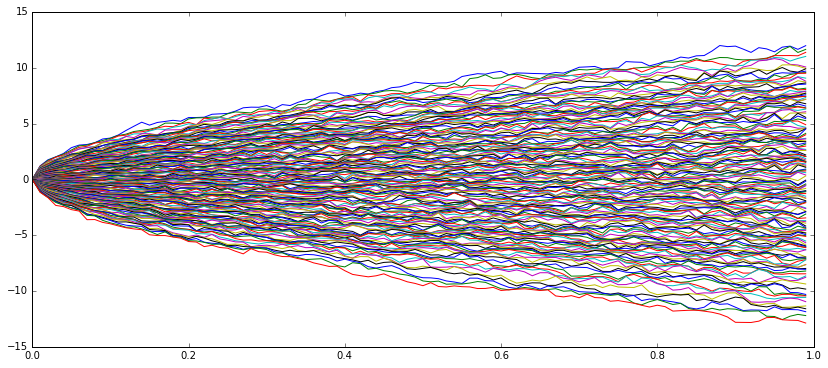
\includegraphics[width=1\textwidth]{images/dyson_brownian_motion.png}
				\caption{\textbf{Eigenvalues trajectories of an Hermitian Brownian motion generated with random matrix SDE.} 50 eigenvalues, with 300 points in$\ [0,1]$ and initial condition $A=0_{\mathcal{M}_N(\mathbb{R})}$.}\label{fig : dyson_brownian_motion}
			\end{figure}\\
			We also note that the eigenvalues seem to "grow" as$\ \sqrt{t}$. Let us explain this observation by the following reasoning. Remember that in Equation \eqref{eq : empirical distribution}, we defined the empirical distribution. Going further, we define the second moment of $\widehat{\mu}_N$
			\begin{equation}
				\widehat{\mu}_{2,N}=\mathbb{E}_{\widehat{\mu}_N}[\lambda^2] = \frac{1}{N}\sum_{i=1}^N\lambda_i^2 \notag
			\end{equation}
			Eigenvalues are function of time, then by taking the expected value we have
			\begin{align}
				\mathbb{E}\left[\frac{1}{N}\sum_{i=1}^N\lambda_i^2(t)\right] = \mathbb{E}\left[\frac{1}{N}Tr(X^2)\right] = \mathbb{E}\left[\frac{1}{N}\sum_{1\leq i,j\leq N}|x_{ij}|^2\right] &= \frac{1}{N}\sum_{1\leq i,j\leq N}\mathbb{E}\left[|x_{ij}|^2\right] \notag\\
				&= \frac{1}{N}\sum_{1\leq i,j\leq N}\frac{t}{N} = t \notag
			\end{align}
			Hence, we represent $\mu_i(t)=\lambda_i(t)/\sqrt{t}$ for $t>0$ on Figure \ref{fig : dbm_rescale}. This renormalisation maintains the trajectories in the interval $[-2,2]$ and allows us to observe the empirical distribution converging to the semicircule law at each time$\ t$ and especially at final time$\ t_f=1$ as the histogram shows.
			\begin{figure}[h] \centering
				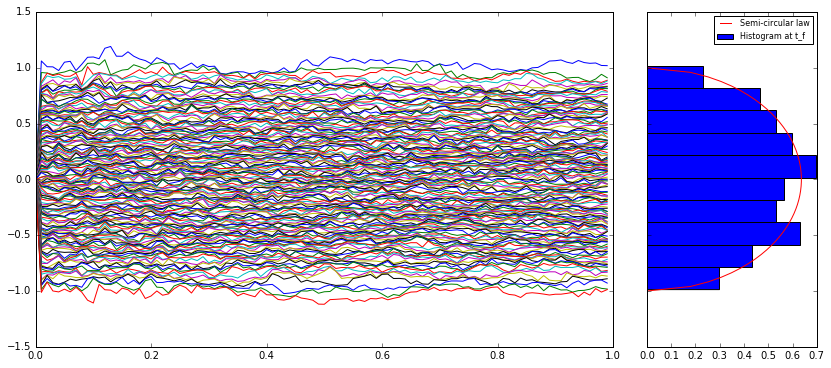
\includegraphics[width=1\textwidth]{images/dyson_brownian_motion_rescaled.png}
			    \caption{\textbf{Rescaled eigenvalues trajectories of an Hermitian Brownian motion generated with random matrix SDE.} 50 eigenvalues, with 300 points in$\ [0,1]$ and initial condition $A=0_{\mathcal{M}_N(\mathbb{R})}$.}\label{fig : dbm_rescale}
			\end{figure}\ \\ \\
			Now that we have a random-matrix process with eigenvalues trajectories, it can be interesting to observe the evolution of the joint distribution of these eigenvalues. Because we know that collection of eigenvalues can have particular properties, we can study the possibility for the static repulsion noticed in Section \ref{sub:determinantal_point_process} to be preserved dynamically by the Hermitian Brownian motion.

		% subsection Random matrix-valued process(end)
		\newpage
		\subsection{Eigenvalues joint distribution at a fixed time} \label{sub:eigenvalues joint distribution over time}
			In this part, we study the evolution of the eigenvalues joint distribution over time. In fact, if this joint distribution has a form adapted to Theorem \ref{th : joh criteria} (e.g. joint distribution of GUE eigenvalues Equation \ref{eq : gue join distrib}), we could find some interesting kernel and characterise the set of eigenvalues at a fixed time as a determinantal point process.\\ \\
			Considering a classical Dyson Brownian motion $\pmb X$ with initial condition $X_0=A$ as decribed in Theorem \ref{dyson-th}, we remark that at each time $t$, $\pmb X $ has \textbf{the same law} as $Y_t=A+t^{1/2}G$ with $G$ a GUE matrix. Considering this observation, the eigenvalues joint distribution is given by the following Theorem, presented in \cite{taotopics,Jo2001}.

			\begin{theorem}\label{th : joint distrib dbm at fixed time}
				Let $A$ be a $N\times N$Hermitian matrix, let$\ t>0$, and let$\ Y_t=A+t^{1/2}G$ where G is drawn from \emph{GUE(N)}. Then if $A$ has a simple spectrum$\ \nu = (\nu_1,...,\nu_N)$, the spectrum$\ \lambda = (\lambda_1,...,\lambda_N)$ of $Y_t$ has probability density function :
				\begin{equation} \label{eq : joint distrib dbm at fixed time}
					\rho_\nu(t,\lambda)=\left(\frac{N}{2\pi t}\right)^{N/2}\frac{\Delta_N(\lambda)}{\Delta_N(\nu)}\det[e^{-\frac{N}{2t}(\lambda_i-\nu_j)^2}]_{i,j=1}^N
				\end{equation}
				on$\ \mathbb{R}_{\geq}^N$, and$\ \Delta_N(\nu) = \prod_{1\leq i<j\leq N}(\nu_i-\nu_j)$ is the Vandermonde determinant.
			\end{theorem}
			The proof of this theorem will not be detailed here but can be easily achieve following \cite{Jo2001} and using our particular distribution of GUE matrices \eqref{eq : GUE distribution}. However, we will focus on the case when $A=0$ and $t=1$. This particular case is not covered by the Theorem \ref{th : joint distrib dbm at fixed time} but we already know that the joint distribution is given by Equation \eqref{eq : gue join distrib} because $Y_1=G$ where $G\sim$ GUE(N).

			Nevertheless, we will check $\lim_{\nu\rightarrow0}\rho_{\nu}(1,\lambda)=u_N(\lambda)$ where $u_N$ is given by Equation \eqref{eq : gue join distrib}, following Exercice 3.1.9. in \cite{taotopics}. An intermediate result concerning the determinant behaviour in this case is presented in the following Lemma.
			\begin{lemma}\label{lem : ex tao}
				Considering $\lambda=(\lambda_1,...,\lambda_N)$ and $\nu=(\nu_1,...,\nu_N)$ as previously defined, we have
				\begin{equation}\label{eq : ex tao 1}
					\det[e^{-\frac{N}{2}(\lambda_i-\nu_j)^2}]_{i,j=1}^N = \prod_{i=1}^Ne^{-N\lambda_i^2/2}\prod_{i=1}^Ne^{-N\nu_j^2/2}\det[e^{N\lambda_i\nu_j}]_{i,j=1}^N
				\end{equation}
				and
				\begin{equation}\label{eq : ex tao 2}
				%\lim_{\nu\rightarrow0}
					\det\left[e^{N\lambda_i\nu_j}\right]_{i,j=1}^N = \frac{N^{\frac{(N-1)N}{2}}}{\prod_{i=1}^N(j-1)!}\Delta_N(\lambda)\Delta_N(\nu)+o(\Delta_N(\nu))
				\end{equation}
			\end{lemma}
			\begin{proof}
			Equation \eqref{eq : ex tao 1} is forthwith
			\begin{align}
				\det[e^{-\frac{N}{2}(\lambda_i-\nu_j)^2}]_{i,j=1}^N &= \det[e^{-N\lambda_i^2/2}e^{-N\nu_j^2/2}e^{N\lambda_i\nu_j}]_{i,j=1}^N \notag \\ 
				&= \prod_{i=1}^Ne^{-N\lambda_i^2/2}\prod_{i=1}^Ne^{-N\nu_j^2/2}\det[e^{N\lambda_i\nu_j}]_{i,j=1}^N \notag
			\end{align}
			Let us now focus on the limit \eqref{eq : ex tao 2}. Using Taylor expansion, we have 
			\begin{align}\label{eq : factor theorem}
				\det\left[e^{N\lambda_i\nu_j}\right]_{i,j=1}^N 
				&= \det\left[\sum_{k=0}^{N-1}\frac{(N\lambda_i\nu_j)^k}{k!} + \sum_{k=N}^{\infty}\frac{(N\lambda_i\nu_j)^k}{k!}\right]_{i,j=1}^N \notag\\
				&= \det(\Lambda V^t + D)\notag \\
				&= \det(C+D)
			\end{align}
			where $\Lambda=\left[\frac{(N\lambda_i)^{j-1}}{(j-1)!}\right]_{i,j=1}^N$, $V=\left[\nu_i^{j-1}\right]_{i,j=1}^N$, $C=\Lambda V^t=[c_{ij}]_{i,j=1}^N$ and \\$D=[o(\nu_j^{N-1})]_{i,j=1}^N=[d_{ij}]_{i,j=1}^N$. \newline
			We denote by $S_N$ the permutation group, and by $\mathcal{P}_N$ the power set of the set $\{1,...,N\}$. When $I\in\mathcal{P}_N$, we note $\overline{I}$ the ensemble $\{1,...,N\}\backslash I$. Using the Leibniz formula, we have
			\begin{align}
				\det(C+D)&=\sum_{\sigma\in S_N} \text{sgn}(\sigma)\prod_{i=1}^N (c_{\sigma(i),i} + d_{\sigma(i),i}) \notag\\
				&=\sum_{\sigma\in S_N} \text{sgn}(\sigma)\sum_{I\in\mathcal{P}_N} \left( \prod_{i\in I} c_{\sigma(i),i} \prod_{i\in\overline{I}} d_{\sigma(i),i}\right) \notag\\
				&= \left(\sum_{\sigma\in S_N} \text{sgn}(\sigma) \prod_{i\in\{1,...,N\}} c_{\sigma(i),i}\right) + \left(\sum_{\sigma\in S_N} \text{sgn}(\sigma) \sum_{I\subsetneq\{1,...,N\}} \prod_{i\in I} c_{\sigma(i),i}\prod_{i\in\overline{I}} d_{\sigma(i),i}\right) \notag \\
				&= \det(C) + \left(\sum_{\sigma\in S_N} \text{sgn}(\sigma) \sum_{I\subsetneq\{1,...,N\}} \prod_{i\in I} c_{\sigma(i),i}\prod_{i\in\overline{I}} d_{\sigma(i),i}\right)
			\end{align}
			Yet, we have
			\begin{align}
				\det(C) = \det(\Lambda N^t) = \det(\Lambda)\det(N^t)&=\det(\Lambda)\det(N) \notag \\
				&= \det\left[\frac{(N\lambda_i)^{j-1}}{(j-1)!}\right]_{i,j=1}^N\det\left[\nu_i^{j-1}\right]_{i,j=1}^N \notag \\
				&= \prod_{j=1}^N\frac{N^{j-1}}{(j-1)!}\det\left[\lambda_i^{j-1}\right]_{i,j=1}^N\det\left[\nu_i^{j-1}\right]_{i,j=1}^N \notag \\
				&=\frac{N^{\frac{(N-1)N}{2}}}{\prod_{j=1}^N(j-1)!}\Delta_N(\lambda)\Delta_N(\nu)\notag
			\end{align}
			Finally, we have to prove 
			\begin{equation*}
				\frac{\det(C+D)}{\Delta_N(\nu)}=\frac{1}{\prod_{i=1}^N(j-1)!}\Delta_N(\lambda)+o(1)
			\end{equation*}
			We found the first term, them we have to prove
			\begin{equation}\label{eq : dernier dernier}
				\frac{1}{\Delta_N(\nu))}\left(\sum_{\sigma\in S_N} \text{sgn}(\sigma) \sum_{I\subsetneq\{1,...,N\}} \prod_{i\in I} c_{\sigma(i),i}\prod_{i\in\overline{I}} d_{\sigma(i),i}\right)=o(1)
			\end{equation}
			This part was not detailed is this study, and we admit Equation \eqref{eq : dernier dernier}. 
			\end{proof}

			Applying Lemma \ref{lem : ex tao} to Theorem \ref{th : joint distrib dbm at fixed time}, we can compute the eigenvalues joint distribution at $t=1$ when $\nu\rightarrow0$
			\begin{equation}\label{eq : joint distrib DBM t=1}
				\rho(1,\lambda)=\left(\frac{N^N}{2\pi}\right)^{N/2}\frac{1}{\prod_{j=1}^N(j-1)!}\Delta_N(\lambda)^2\prod_{i=1}^Ne^{-\lambda_i^2/2} 
			\end{equation}
			Which is exactly the joint distribution of GUE matrices, see Equation \eqref{eq : gue join distrib}. Hence, at $t=1$, we can apply every result on GUE matrices highlighted in Section \ref{sec:static_random_matrices_and_eigenvalues}. Actually, the collection of eigenvalues at $t=1$ of a Hermitian Brownian motion is a determinantal point process, with kernel given in Theorem \ref{th : kernel eig GUE}. This is undoubtely an interesting result, however it is only valid for $t=1$. Later, Section \ref{subsect : O-U process intro} will present a model, slightly different from the Hermitian Brownian motion, able to preserve the GUE distribution at each time when $t\rightarrow+\infty$.\\ \\
			This section and the previous one motivate the analysis of the eigenvalues processes generated by the Hermitian Brownian motion. Nevertheless, one can imagine a way to simulate directly the eigenvalues processes, without considering any matrix-valued random process. Next section spotlight a fundamental result related to this remark.


		\subsection{Random matrix SDE and associated eigenvalues SDEs}\label{subsection : DBM matrix - ev}

			After this brief introduction of some useful definitions and concepts for this study, we now present the most classical process correponding to our context : the Dyson Brownian motion. The first step in the Dyson Brownian motion presentation highlights the link between random matrix SDE and system of eigenvalues SDEs, following \cite{taotopics,agz}.

			The classical Dyson Brownian motion is defined as follows in Theorem \ref{dyson-th}.
			\begin{theorem}[Dyson Brownian motion]\label{dyson-th}
				Let A be a $N\times N$ Hermitian matrix and $\pmb X$ the matrix-valued process defined by $X_t=A+H_t$ with $\pmb H$ a $N \times N$ Hermitian Brownian motion. The eigenvalues$\ \{\lambda_1(t),...,\lambda_N(t)\}$ of $\pmb X$ are almost surely distinct. Ordering $(\lambda_i(t))_{1\leq i\leq N}$ so that $\lambda_1(t)<\lambda_2(t)<...<\lambda_{N-1}(t)<\lambda_N(t)$ for $t>0$, they satisfy the following system of SDEs : 
				\begin{align}\label{eq : dyson-for}
					d\lambda_i(t)=
					\frac{1}{\sqrt{N}}dw_i(t) + \frac{1}{N}\sum_{\substack{j=1 \\ j \neq i}}^N\frac{1}{\lambda_i(t)-\lambda_j(t)}dt
				\end{align}
				with$\ (w_{i}(t))_{1\leq i\leq N}$ a collection of independent real standard Brownian motions and initial conditions $(\lambda_i(0))_{1\leq i\leq N}$ the eigenvalues of $A$ so that $\lambda_1(0)\leq\lambda_2(0)\leq...\leq\lambda_{N-1}(0)\leq\lambda_N(0)$.
			\end{theorem}
			This theorem is proved in \cite{agz,taotopics} and we will give an idea of proof following \cite{taotopics} and the proof of a more general theorem following \cite{grac} in Chapter 2.

			\begin{remark}\label{rem: dyson_eigen}
				Unlike in Remark \ref{rem: SDE first def}, Equation \eqref{eq : dyson-for} is now a scalar SDE. Let assume that a scalar SDE is just an initial condition, a Brownian increment and a \textit{drift}. In Section \ref{subsect : O-U process intro}, we will give a more general definition of scalar SDEs.\\
				The solution of a SDE as described in Equation \eqref{eq : dyson-for} are called \textit{diffusions}. Let us try to understand the role of the two terms appearing in Equation \eqref{eq : dyson-for}. The first one represents the term of diffusion, and it is remarkable that the \textit{coefficient of diffusion} is a constant $1/\sqrt{N}$. The second - corresponding to the drift - introduces an noticeable idea of \textit{repulsion} between the eigenvalue, which recall the repulsion presented in Section \ref{sub:determinantal_point_process}.
			\end{remark}
			
			This last result allows us to consider the second way of generating the eigenvalues trajectories : the simulation using the eigenvalues system of SDEs. Instead of having a random matrix SDE, here we have got a system of$\ N$ scalar SDEs satisfied by the eigenvalues of a random matrix-valued process (a.k.a. the Hermitian Brownian motion).\\ \\
			However, we cannot have the same guarantee provided by Lemma \ref{th : HBM increments} for Algorithm \ref{alg: random mat SDE}. In this second case, we have to use an Euler discretisation (see \cite{kloeden2012numerical}, Chapitre 9) to simulate these trajectories which make these simulations \textbf{approximate} and no longer exact. Algorithm \ref{alg: dbm eigenvalues SDE} explains how these simulations have been performed and is also available on \cite{sebastienGithub}.
			
			\begin{algorithm}[H]
					\begin{algorithmic}
					\STATE \textbf{input :} $A,\ N,\ n_{samples},\ t_f$
					\STATE \textbf{initialisation :}
					\STATE $dt\leftarrow t_f/n_{samples}$ 
					\STATE $\Lambda \leftarrow \{OrderedSpectrum(A)\}$
					\FOR{t=1 \textbf{to}$\ n_{sample}$}
					\FOR{i=1 \textbf{to} N}
					\STATE draw$\ B\sim \mathcal{N}(0,1)$
					\STATE $D\leftarrow\frac{1}{N}\sum_{j\neq i}\frac{1}{\Lambda(t,i)-\Lambda(t,j)}$
					\STATE $\Lambda(t+1,i) \leftarrow \Lambda(t,i) + \sqrt{dt/N}*B+D*dt$
					\ENDFOR
					\ENDFOR
					\STATE \textbf{output :} $\Lambda$
					\end{algorithmic}
					\caption{Eigenvalues trajectories simulation with system of eigenvalues SDEs}
					\label{alg: dbm eigenvalues SDE}
			\end{algorithm}
			Equally to Algorithm \ref{alg: random mat SDE}, by transforming$\ \Lambda$ into a$\ N\times n_{samples}$ matrix, each row represent the value of an eigenvalue over time.\newline


			Figure \ref{fig : dbm_eigenvalues} shows 50 eigenvalues processes, simulated using their SDE.
			\begin{figure}[h!] 
				\includegraphics[width=1\textwidth]{images/dbm_eigenvalues_50_3000.png}
			    \caption{\textbf{Eigenvalues trajectories generated with the Dyson Brownian motion eigenvalues system of SDEs.} 50 eigenvalues, with 3000 points in$\ [0,1]$.} \label{fig : dbm_eigenvalues}
			\end{figure}
			Unfortunately, because of the approximate nature of these simulations, we can observe some "jumps" of trajectories. These jumps are due to the Euler discretisation created to generate them. Indeed, the generation of these trajectories needs the computation of$\ d\lambda_i(t)$ at each step and for$\ i \in\{i,...n\}$, then add these increments to the current values$\ \lambda_i(t)$. However, these computations are obtained separatedly and cannot guarantee each trajectory to not intersect with others. Consequently, after an intersection we observe a "jump". This phenomenom can be limited by using a very thin discretisation (i.e. fixing $dt$ to a very small value) and by initialising eigenvalues not too close to each other - as in Figure \ref{fig : dbm_eigenvalues} - but it cannot be fully avoided.\\ \\
			We can still quickly comment simulations using the random matrix SDE and using the system of eigenvalues SDEs. Indeed, these two methods provide a way to compute the eigenvalues trajectories by defining discretisation policy - choosing $n_{samples}$ and $t_f$. Let us remark that if we have the system of eigenvalues SDEs corresponding to a random matrix SDE, this second method is far less computationaly costly than the first one, as Table \ref{tab : comparison 1} shows.
			\begin{table}[h]
	   			\centering
				  \begin{tabular}{|l|c|c|}
				    \cline{2-3}
				    \multicolumn{1}{c|}{} & Matrix SDE & Eigenvalues SDEs \\ \hline
				    Type of simulation & Exact  & Approximate  \\ \hline
				    $\#$ simulations $\sim\mathcal N$ & $2N^2$ &  $N$ \\ \hline
				    Diagonalisation & $O(N^3)$   & None  \\ \hline
				    Robustness & High & Low ("jumps") \\ \hline 
				  \end{tabular}
				\caption{Comparison of the two simulation methods}\label{tab : comparison 1}	
			\end{table}\\
			First because we only need $N$ generations of random variables following a normal distribution and secondly because we do not need to diagonalise at each step. However, this simulation method is less robust than the simulation with the random matrix SDE.
			To conclude, it seems that there is not a perfect method but the choice between the one or the other can depend on the application. Still, the link between both is complex and will motivate the following questioning.\\ \\
			After this complete presentation of the Dyson Brownian motion we will now focus on other examples of these type of processes. In fact, the Dyson Brownian motion is a starting point and several other processes derived from it. In this study, we choose to present two other particular processes : the Ornstein-Ulhenbeck process and the Wishart process.
		% subsection eigenvalues_system_of_sdes (end)
	
	% section the_dyson_brownian_motion (end)

	\newpage
	\section{Other classical examples}
		The two other examples exposed here have different interesting properties. The first one, the Ornstein Ulhenbeck process is remarkable because it is preserve the GUE distribution at each time $t$. Otherwise, the Wishart is notable because it generates only non-negative trajectories which can be attractive for some simulations.\\
		Note that every simulations in this part had been performed using algorithms available on \cite{sebastienGithub}.
		\subsection{The Ornstein-Ulhenbeck process}\label{subsect : O-U process intro}
 			The previous part aims to consider a matricial form of the Brownian motion and leads us to analyze the Dyson Brownian motion. In this part we try to reproduce this analysis with another simple example : the Ornstein-Ulhenbeck process. However, we need to go further in the definition of scalar and matrix Stochastic Differential Equations because this example is slightly more complicated than the Dyson Brownian motion.\\
 			Thus, introducing the Ornstein-Ulhenbeck process gives us the opportunity to remind some few points concerning SDEs. There is a wide development of SDEs in the literaturea and the reader can refer to \cite{simonsto,oksendal2003stochastic} for instance.

			\subsubsection{Stochastic Differential Equations}
			In order to understand the motivation of SDEs, let us start by considering an Ordinary Differential Equation namely a system
			\begin{equation*} \left\{
				\begin{array}{ll}
	        		\frac{dz}{dt}=b(t,z(t))\\
	        		z(0) = u 
	    		\end{array}\right.\notag
			\end{equation*}
			where $z : \mathbb{R}^+\rightarrow \mathbb{R}$ is the unknown function and $b : \mathbb{R}^+\times\mathbb{R}\rightarrow\mathbb{R}$ is a given function. Now, imagine that we want a "noisy" version of this previous equation. The simplest way to do that is by adding a Brownian motion. However, because the Brownian motion is almost surely non derivable, we define the Stochastic Differential Equation as follows
			\begin{equation} \label{eq : SDE general}
				Z(t) = u +\int_0^tb(s,Z(s))\ ds + \sigma (B(t))
			\end{equation}
			with $\sigma \in \mathbb{R}$ corresponding to the diffusion coefficient and $(B(t))_{t\geq 0}$ a real Brownian motion. Recall that $(Z(t))_{t\geq 0}$ is now a scalar-valued random process. This is the integral form of SDEs, and the only form which is mathematically correct. Nevertheless, the following notation is generally used to point this SDE
			\begin{equation*} \left\{
				\begin{array}{ll}
	        		dZ(t)=b(t,Z(t))\ dt+\sigma dB(t)\\
	        		Z(0) = u 
	    		\end{array}\right.\notag
			\end{equation*}
			\begin{remark}\label{rem: drift dep on time}
				Stochastic Differential Equations are usually defined in a more general context, where $\sigma$ is a function of the time and the process. Here we will only develop the case related to the Ornstein-Ulhenbeck process so that the reader can intuitively understand SDEs and because we did not introduce It\^{o} integral so far. It\^{o} calculus will only be introduced in section \ref{subsect : ito formula}, for the need of the proof on Theorem \ref{gen_th}.
			\end{remark}
			Focusing on the particular process studied in this part, the Ornstein-Ulhenbeck process is the solution of this equation, namely the \textit{Langevin equation}
			\begin{equation}\label{eq : langevin scalar}
				Z(t) = U - a\int_0^tZ(s)\ ds+\sigma B(t) 
			\end{equation}
			where $a, \sigma \in \mathbb{R}$, $Z(0)=U$ a random variable and $(B(t))_{t\geq 0}$ a real Brownian motion independent from $U$. We can write this equation as follows
			\begin{equation*} \left\{
				\begin{array}{ll}
	        		dZ(t)=-aZ(t)\ dt+\sigma dB(t)\\
	        		Z(0) = U
	    		\end{array}\right.\notag
			\end{equation*}
			In the particular case where $U \sim\mathcal N(m,\sigma_0^2)$ independent of $(B(t))_{t\geq 0}$, we have the following result 
			\begin{proposition}\label{prop : solution langevin scalar}
			The Langevin equation \eqref{eq : langevin scalar} has a unique solution given by
			\begin{equation}\label{eq : langevin scalar solution}
				Z(t)=e^{-at}\left(U+\sigma\int_0^te^{as}dB(s)\right)
			\end{equation}
			Assuming that $U \sim\mathcal N(m,\sigma_0^2)$ independent of $(B(t))_{t\geq 0}$, $(Z(t))_{t\geq0}$ is a Gaussian process of expected value 
			\begin{equation}
				\mathbb{E}[Z(t)]=me^{-at}\notag
			\end{equation}
			and covariance function
			\begin{equation}
				\mathrm{Cov}(Z(s), Z(t))=e^{-a(t+s)}\left(\sigma_0^2+\frac{\sigma^2}{2a}(e^{2a(s\wedge t)}-1)\right) \notag
			\end{equation}
			with $t,s\geq 0$ and $s\wedge t=min(s,t)$.
			\end{proposition}
			By showing that $(Z(t))_{t\geq0}$ is a Gaussian process, we implicitly explain that the solution of Langevin equation preserves the normal random distribution when $t\rightarrow\infty$. This result will have its matrix equivalent later (Proposition \ref{prop : solution langevin matricial}). Let us give a proof of the expression of the expected value and the covariance function.
			\begin{proof}
				The solution of the Langevin equation \eqref{eq : langevin scalar solution} is admitted.\\
				We know that $t\rightarrow e^{-at}U$ is a Gaussian process. Then, by the properties of the It\^{o} integral,
				\[t\rightarrow\sigma\int_0^te^{-a(t-s)}dB(s)\] is also a Gaussian process with zero expected value. Hence, $(Z(t))_{t\geq0}$ which is the sum of the two previous processes is also a Gaussian process of expected value
				\begin{equation}
					\mathbb{E}[Z(t)]=\mathbb{E}[e^{-at}U]=e^{-at}\mathbb{E}[U]=me^{-at} \notag
				\end{equation}
				Regarding the covariance function and using the isometry property of the It\^{o} integral we have
				\begin{align}
					\mathrm{Cov}(Z(s),Z(t))&=\mathrm{Cov}(Ue^{-as},Ue^{-at})+\mathrm{Cov}\left(\sigma\int_0^se^{a(v-s)}dB(u),\sigma\int_0^te^{a(v-t)}dB(v)\right)\notag\\
					&=e^{-a(t+s)}\left(\mathrm{Var}(U)+\sigma^2\int_0^{s\wedge t}e^{2av}dv\right)\notag\\
					&=e^{-a(t+s)}\left(\sigma_0^2+\frac{\sigma^2}{2a}(e^{2a(s\wedge t)}-1)\right) \notag
				\end{align}
			\end{proof}
			The reader must notice that the classical Langevin equation is define for real scalar-valued stochastic processes. Hence, it can be extended to matrix-valued processes. Then, we define the Langevin equation for the matrix-valued random process $\pmb X$ as
			\begin{equation}\label{eq : langevin mat}
				X_t = U - a\int_0^tX_s\ ds+H_t
			\end{equation}
			or equally
			\begin{equation} \left\{
				\begin{array}{ll}
	        		X_0 = U \\
	        		dX_t=-aX_t\ dt+dH_t
	    		\end{array}\right.\notag
			\end{equation}
			where $b\in \mathbb{R}$, $X_0=U$ a random matrix and $\pmb H$ a Hermitian Brownian motion as defined in Definition \ref{herm-mat-def} and independent from $U$. Here, the solution of the SDE \eqref{eq : langevin mat} will no longer be a real-valued process but a $N\times N$ matrix-valued process. As mentioned above, Proposition \ref{prop : solution langevin scalar} has its parallel for matrix-valued process, as Proposition \ref{prop : solution langevin matricial} shows.

			\begin{proposition}\label{prop : solution langevin matricial}
			The Langevin equation \eqref{eq : langevin mat} has a unique solution $\pmb X$ and if $U\sim$ \emph{GUE(N)} and $a=1/2$, then $X_t\sim$ \emph{GUE(N)} when $t\geq0$
			\end{proposition}

			\begin{proof}
			Let us now assume that $U\sim$ GUE(N) (see Definition \ref{gue-mat-def}) and observe the behaviour of the entries $\pmb X_{kl}$ with $k,l\in\{1,...,N\}$.\\
			Equation \eqref{eq : langevin mat} means that every diagonal entries of $\pmb X_{kk}$ is a Gaussian process, verifying \eqref{eq : langevin scalar} with $\sigma = 1/\sqrt{N}$. Using Proposition \ref{prop : solution langevin scalar} we have
			\begin{align}
				\mathbb{E}[X_{kk,t}]&=0\notag \\
				\mathrm{Var}(X_{kk,t})=\mathrm{Cov}(X_{kk,t},X_{kk,t})&=\frac{1}{N}e^{-2at}+\frac{1}{2aN}(1-e^{-2at})\notag
			\end{align}
			Because we set $a=1/2$, we have $X_{kk,t}\sim\mathcal{N}_\mathbb R(0,1/N)$.\\
			Moreover, every entries above the diagonal - when $k<l$ - has its real part and imaginary part verifying \eqref{eq : langevin scalar} with $\sigma = 1/\sqrt{2N}$ (recall that the two Brownians in the definition of the Hermitian Brownian motion are independent, see \ref{herm-mat-def}). It means that
			\begin{align}
				\mathbb{E}\left[\mathrm{Re}(X_{kl,t})\right]&=0\notag \\
				\mathrm{Var}\left(\mathrm{Re}(X_{kl,t})\right)=\mathrm{Cov}\left(\mathrm{Re}(X_{kl,t}),\mathrm{Re}(X_{kl,t})\right)&=\frac{1}{2N}e^{-2at}+\frac{1}{4aN}(1-e^{-2at})\notag
			\end{align}
			and the same equations for the imaginary part. Hence, for $1<k<l<N$ with $a=1/2$, we have $\mathrm{Re}(X_{kl,t})\sim\mathcal{N}_\mathbb R(0,1/2N)$ and $\mathrm{Im}(X_{kl,t})\sim\mathcal{N}_\mathbb R(0,1/2N)$. \\
			Finally, $X_{kl,t}\sim\mathcal{N}_\mathbb C(0,1/N)$ for $1<k<l<N$ and $X_t\sim$ \text{GUE(N)}.
			\end{proof}

			This proposition allows us to directly apply results from the first part such as Theorems \ref{th : wigner}, \ref{th : joint distrib GUE} and \ref{th : kernel eig GUE} because it ensures the solution of the matrix Langevin equation to preserve the GUE ensemble. With this proposition, we finally find a matrix-valued process which can preserve a particular distribution of matrices (Equation \eqref{eq : GUE distribution}) at each time $t$, involving that the eigenvalues joint distribution (Equation \eqref{eq : gue join distrib}) also hold and even that the collection of eigenvalues at a fixed time is a determinantal point process (with kernel given by Equation \eqref{eq : kernel GUE}).
			\\ \\
			After this brief point on SDEs, we now explain the link between random matrix SDE \eqref{eq : langevin mat} and SDEs of their eigenvalues - as we have done with the Dyson Brownian motion - in the particular case where $a=1/2$.


			\subsubsection{Random matrix SDE and associated eigenvalues SDEs}
				In this part, we will use quite the same notation as in \cite{agz}. One can refer to Exercice 4.3.9 in \cite{agz}. This result will be presented as a theorem.

				\begin{theorem}[Ornstein-Ulhenbeck process]\label{orn-ulh-th}
					Let A be a $N\times N$ Hermitian matrix and $\pmb X$ the matrix-valued process solution of the stochastic differential equation$\ dX_t=dH_t-\frac{1}{2}X_t\ dt$ with $\pmb H$ an Hermitian Brownian motion and $X_0=A$. The eigenvalues $\{\lambda_1(t),...,\lambda_N(t)\}$ of $\pmb X$ are almost surely disctint. Ordering $(\lambda_i(t))_{1\leq i\leq N}$ so that $\lambda_1(t)<\lambda_2(t)<...<\lambda_{N-1}(t)<\lambda_N(t)$ for $t>0$, they satisfy the following system of SDE : 
					\begin{align}\label{eq : orn-ulh-eq}
						d\lambda_i(t)=
						\frac{1}{\sqrt{N}}dw_i(t) + \frac{1}{N}\sum_{\substack{j=1 \\ j \neq i}}^N\frac{1}{\lambda_i(t)-\lambda_j(t)}dt -\frac{1}{2}\lambda_i(t)dt
					\end{align}
					with$\ (w_{i}(t))_{1\leq i\leq N}$ a collection of independent real standard Brownian motions and initial conditions $(\lambda_i(0))_{1\leq i\leq N}$ the eigenvalues of $A$ so that $\lambda_1(0)\leq\lambda_2(0)\leq...\leq\lambda_{N-1}(0)\leq\lambda_N(0)$.
				\end{theorem}
				By comparing the two systems of SDEs \eqref{eq : dyson-for} and \eqref{eq : orn-ulh-eq}, note that the drift is now formed by two terms. This second new term influence the eigenvalues trajectories by limiting their growths. It makes the process solution of SDE stronger than the classical Dyson Brownian motion in the sense that the dynamic does not only preserve the eigenvalues empirical distribution. The dynamic also preserves the eigenvalues joint distribution of the GUE - and for all $t$ when $t\rightarrow+\infty$, not only for $t=1$ (see Equation \eqref{eq : joint distrib DBM t=1}).

			\paragraph{Simulation with random matrix SDE}
				When we represent the evolution of this process and the empirical distribution at a fixed time $t$, we can clearly observe the semicircule law. An example is presented on Figure \ref{fig : orn-ulh}, where the empirical distribution is plotted for $t_f=1$.
				\begin{figure}[h] 
					\includegraphics[width=1\textwidth]{images/ornstein_ulhenbeck_histo.png}
				    \caption{\textbf{Eigenvalues trajectories of a Ornstein-Ulhenbeck process generated by random matrix SDE.} 50 eigenvalues, with 300 points in$\ [0,1]$.} \label{fig : orn-ulh}
				\end{figure}

			\paragraph{Simulation with eigenvalues SDEs}
				As we do for the Dyson Brownian motion, we try to simulate these trajectories using the eigenvalues SDEs instead of the random matrix SDE. Results are shown on Figure \ref{fig : orn-ulh-50}. \newline
				\begin{figure}[h!] 
					\includegraphics[width=1\textwidth]{images/orn_ulh_eigenvalues_histo_30_3000.png}
				    \caption{\textbf{Eigenvalues trajectories of a Ornstein-Ulhenbeck process generated by eigenvalues SDEs.} 30 eigenvalues, with 3000 points in$\ [0,1]$.} \label{fig : orn-ulh-50}
				\end{figure}

				The semicircule law seems to appear at final time$\ t_f$. However with only 50 trajectories, it is difficult to represent a valid histogram. Unfortunately, when we decide to increase the number of trajectories, it creates some "jumps" on several trajectories as Figure \ref{fig : orn-ulh-100} shows. \newline
				This phenomenom was observed on Figure \ref{fig : dbm_eigenvalues} and explained in the previous part. This can be limited by using a very thin discretisation, like on Figure \ref{fig : orn-ulh-100} where we multiply the number of points in $[0,1]$ by 10.
				\begin{figure}[h!] 
					\includegraphics[width=1\textwidth]{images/orn_ulh_eigenvalues_histo_100_3000.png}
				    \caption{\textbf{Eigenvalues trajectories of a Ornstein-Ulhenbeck process generated by eigenvalues SDEs.} 100 eigenvalues, with 3000 points in$\ [0,1]$.} \label{fig : orn-ulh-100}
				\end{figure}


		\subsection{The Wishart process}
			As it was shortly introduce at the beginning of this section, we decide to present the Wishart process. This process is rather different from the Dyson Brownian motion and the Ornstein-Ulhenbeck process because it no longuer have something to do with GUE matrices. However, the Wishart process has the particularity to preserve non-negative eigenvalues trajectories. Thus, the joint distribution will be specific, and the determinant point process formed by the collection of eigenvalues at a fixed time $t$ too. 

			\subsubsection{Eigenvalues joint distribution and determinantal point process} % (fold)
			\label{sub:eigenvalues_joint_distribution_and_determinantal_point_process}
				Before explicitly defining the Wishart process, we have to present the joint distribution of the Wishart matrix ensemble, and the kernel of the determinantal point process.
				\begin{theorem}[Eigenvalues joint distribution and DPP kernel for Wishart matrices]
					Let $V$ be a $M\times N$ matrix with $M\leq M$ with entries $V_{ij}\sim \mathcal N_\mathbb C(0,1)$ for $1\leq i\leq M$ and $1\leq j\leq N$.\\
					We fix the reference measure to $\mu(dx)=x^{N-M}e^{-x}\mathds{1}_{[0,+\infty[}(x)dx$, the eigenvalues joint distribution of $V^*V$ is given by 
					\[\frac{1}{Z_N}\prod_{i<j}(x_i-x_j)^2\mu^{\otimes N}(dx) \]
					with $Z_N$ a normalisation constant.\\
					The point process $\{\lambda_1,...\lambda_N\}$ associated with the eigenvalues of $V^*V$ is determinantal with kernel
					\[K_N(x,y)=\sum_{i=0}^{N-1}\frac{l_i(x)l_i(y)}{||l_i||^2}x^{\frac{N-M}{2}}y^{\frac{N-M}{2}}e^{-\frac{x+y}{2}}\mathds{1}_{[0,+\infty[\times[0,+\infty[}(x,y)\]
					with $(l_i)_{0\leq i\leq N-1}$ the orthogonal polynomial with respect to the measure $\mu$ (a.k.a the Laguerre polynomials with parameter $N-M$).
				\end{theorem}
				\begin{proof} Not detailed here, but very close to the proof of Theorem \ref{th : kernel eig GUE}.
				\end{proof}
				Let us now introduce the Wishart process, able to preserve the Wishart matrix distribution over time.

			% subsection eigenvalues_joint_distribution_and_determinantal_point_process (end)

			\subsubsection{Random matrix SDE and associated eigenvalues SDES}
			For this result, we refer to Exercice 4.3.8 in \cite{agz}. and present it as a theorem.
			\begin{theorem}[Wishart process]\label{wish}
				Let $\pmb V$ be a $M\times N$ matrix whose entries are independent complex Brownian motions and let$\ V_0$ be a $M\times N$ matrix with complex entries. The eigenvalues $\{\lambda_1(t),...,\lambda_N(t)\}$ of $\pmb X$ defined by $X_t=V_t^*V_t$ are almost surely distinct. Ordering $(\lambda_i(t))_{1\leq i\leq N}$ so that $\lambda_1(t)<\lambda_2(t)<...<\lambda_{N-1}(t)<\lambda_N(t)$ for $t>0$, they satisfy the following system of SDE :
				\begin{align}
					d\lambda_i(t)=
					2\sqrt{\frac{\lambda_i(t)}{N}}dw_i(t) + 2\left(\frac{M}{N}+\frac{1}{N}\sum_{\substack{j=1 \\ j \neq i}}^N\frac{\lambda_j(t)+\lambda_i(t)}{\lambda_i(t)-\lambda_j(t)}\right)dt
				\end{align}
				with$\ (w_{i}(t))_{1\leq i\leq N}$ a collection of independent real standard Brownian motions and initial conditions $(\lambda_i(0))_{1\leq i\leq N}$ the eigenvalues of $V_0^*V_0$ so that $\lambda_1(0)\leq\lambda_2(0)\leq...\leq\lambda_{N-1}(0)\leq\lambda_N(0)$.
			\end{theorem}
			Considering the definition of the eigenvalues$\ (\lambda_i(t))_{1\leq i\leq N}$, we can remark that they are define as eigenvalues of the covariance matrix of$\ (X_t)_{t\geq 0}$. Thus, eigenvalues of Wishart matrices are non negative.

			\begin{remark}[Random matrix SDE]\label{rem : wish mat process}
				This theorem does not explicitly present the SDE verified by the matrix-valued process $\pmb X$. Referring to \cite{grac} - this reference will be widely used in Section \ref{sec : graczyk dem}, we explain it : with the conditions of Theorem \ref{wish}, the process $\pmb X$ is the solution of the random matrix SDE 
				\begin{equation} \left\{
					\begin{array}{ll}
		        		dX_t = \sqrt{\frac{1}{N}}\sqrt{X_t}dB_t +\sqrt{\frac{1}{N}} dB_t^*\sqrt{X_t}+\frac{2M}{N}Idt\\
		        		X_0=V_0^*V_0 
		    		\end{array}\right.\notag
				\end{equation}
				with $\pmb B$ a $N\times N$ complex Brownian motion and $V_0$ be a $M\times N$ matrix with complex entries. The expression of this SDE will be more detailed in Section \ref{sec : gen th applied to ex}.
			\end{remark}

			\paragraph{Simulation with the matrix-valued process}
			For this particular simulation, we do not use the SDE presented in Remark \ref{rem : wish mat process}, because we prefer to generate $\pmb V$ and compute $\pmb X$ at each step with $X_t=V_t^*V_t$. The sign of the eigenvalues (see Figure \ref{fig : wish}) generates a slightly different representation from the two previous examples. Due to this process, we manage to generate $N$ Brownian motions conditioned to avoid collision, which take only positive values.
			\begin{figure}[h!] 
				\includegraphics[width=1\textwidth]{images/wishart.png}
			    \caption{\textbf{Eigenvalues trajectories of a Wishart process generated with the matrix-valued process.} 30 eigenvalues, with 100 points in$\ [0,1]$ and $\ M=25$.} \label{fig : wish}
			\end{figure}

			\paragraph{Simulation with eigenvalues SDEs}
			Unfortunately, when we try to simulate Wishart processes using the eigenvalues SDEs, we observe that it is very difficult to maintain the eigenvalues non negative. In fact, simulations fail because of the computation of the square root of a negative real. We are not able to present result of the generation of a Wishart process using eigenvalues SDEs. \vspace{1cm}

			At the end of this chapter of examples, we can conclude that eigenvalues processes of matrix-valued random process have the property to dynamically preserve a repulsion, by preserving a DPP. Thanks to these time processes, we have an interesting way of simulate them.\\
			Moreover, it is clearly more robust to simulate these type of processes with associated random matrix SDEs than with systems of eigenvalues SDEs. Simulating with the system of eigenvalues SDEs was barely acceptable with the Ornstein-Ulhenbeck process but not possible with the Wishart process. Simulations from random matrices are finally more robust and easier to pratice, while they are more computationally costly and less interpretable than simulations with eigenvalues SDEs. In a perfect world, we would like to think the simulation in term of a system of eigenvalues SDEs and run it with the associated random matrix SDE.\newline

			Having a clear understanding of the link between these two aspects of the same problem is crucial and we will try to enlighten it in the following section.


%\strut
%\newpage

\chapter{Matrix and eigenvalues stochastic differential equations}\label{chap 2}
	This chapter is mainly dedicated to give an intuition of the relations between random matrix SDE and eigenvalues SDEs. In the most simple case - the Dyson Brownian motion - this link is described by Theorem \ref{dyson-th}. A proof of this theorem is given in \cite{taotopics} using a particular approach based on the Hadamard's formulas. \newline
	In the first section, we try to apply the same approach to prove Theorem \ref{orn-ulh-th} and we will see that this method is finally limited and can only give us a \textbf{heuristic} to prove this result. The second section will focus on another approach following \cite{grac} which gives a general theorem to link random matrix SDE and associated system of eigenvalues SDEs in a very general case.

	\section{Hadamard formulas approach}\label{section : hadamard approach}
		To prove Theorem \ref{orn-ulh-th}, following \cite{taotopics}, we first need to introduce and prove the Hadamard's first and second variation formulas.

		\subsection{Hadamard's first and second variation formulas}
			Let us consider a \textbf{deterministic} Hermitian matrix-valued process $\pmb A$ with simple spectrum and with all of its coefficients $(a_{ij}(t))_{0\leq i,j\leq n}$ twice derivable functions of variable $t$. Then, we define $\pmb{\dot A}$ and $\pmb{\ddot A}$ with entries respectively defined by $\dot a_{ij}(t)=da_{ij}/dt$ and $ \ddot a_{ij}(t)=d^2a_{ij}/dt^2$ for $i,j \in \{1,...,N\}$. Because $\pmb A$ has a simple spectrum, we can clearly define $N$ trajectories and number them from 1 to $N$ thereby $\lambda_1(t)<\lambda_2(t)<...<\lambda_{N-1}(t)<\lambda_N(t)$ for $t\geq0$.
			It is also known that the eigenvalues processes $(\lambda_i(t))_{0\leq i\leq n}$ and the associated eigenvectors $(u_i(t))_{0\leq i\leq n}$ of $\pmb A$ are twice derivable.


			For $i\in \{1,...,N\}$, the Hadamard's first and second variation formulas are useful to link the derivative of an eigenvalue process of $\pmb A$, denoted $(\lambda_i(t))_{t\geq0}$ defined by $\dot\lambda_i (t) = d\lambda_i/dt$ and $\ddot\lambda_i (t) = d^2\lambda_i/dt^2$ to $\pmb{\dot A}$ and $\pmb{\ddot A}$.
			

			\begin{lemma}[Hadamard's first variation formula]\label{had1}
				Let $\pmb A$ be a $N\times N$ Hermitian matrix-valued process with simple spectrum. Suppose that $\pmb A$ is a derivable function of $t$. Denote by $(\lambda(t))_{t\geq 0}$ an eigenvalue of $\pmb A$ and $u=(u(t))_{t\geq 0}$ its associated eigenvector, we have :
				\begin{align}\label{had1-for}
					\dot{\lambda}(t) = u^*\dot{A_t}u
				\end{align}
				for $t\geq 0$.
			\end{lemma}

			\begin{proof}
				See appendix \ref{hadamard1}.
			\end{proof}


			\begin{lemma}[Hadamard's second variation formula]\label{had2}
				Let $\pmb A$ be a $N\times N$ Hermitian matrix-valued process with simple spectrum.. Suppose that $\pmb A$ is a twice derivable function of $t$. We denote by $(\lambda_i(t))_{1\leq i\leq N}$ the eigenvalues of $\pmb A$ and $u_i=(u_i(t))_{1\leq i\leq N}$  their associated eigenvectors for $t\geq0$. For$\ 1\leq i \leq N$ and $t\geq0$, we have
				\begin{align} \label{had2-for}
					\ddot{\lambda_i}(t) =u_i^*\ddot{A_t}u_i + 2\sum_{\substack{j=1 \\ j \neq i}}^{n} \frac{| u_{j}^*\dot{A_t}u_i |^2}{\lambda_i(t)-\lambda_j(t)}
				\end{align}
			\end{lemma}

			\begin{proof}
				See appendix \ref{hadamard2}.
			\end{proof}

			\begin{remark}
			Here one can make a very astonishing observation. The equation \eqref{had2-for} in lemma \ref{had2} shows the interaction between the eigenvalues even if there is not any randomness in the theorem. Repulsion between eigenvalues seems to be more general: it is an "algebric repulsion", also remarkable for matrices satisfying Ordinary Differential Equations.
			\end{remark}


		\subsection{The Ornstein-Ulhenbeck process using Hadamard's approach}
			In this section, we give a \textbf{heuristic} for Theorem \ref{orn-ulh-th} using a Taylor expansion and the Hadamard's variation formulas \eqref{had1-for} and \eqref{had2-for}. The following development is not rigourous and cannot establish an exact proof. However, these computations are still relevant because it gives us an intuition of the eigenvalues SDEs setting up.\\
			Note that the $i$th eigenvector will be noted $u_i$ for notation simplification but the reader must remember that $u_i$ depends on the time i.e. $u_i=(u_i(t))_{1\leq i\leq N}$.

			\begin{proof}[Heuristic of \ref{orn-ulh-th} using a Taylor expansion and the Hadamard variation formulas]

			Let $\pmb H$ be an Hermitian Brownian motion and $\pmb X$ be the matrix-valued process solution of the stochastic differential system:
			\begin{align}\label{eq : sde-mat}
				dX_t=dH_t-\frac{1}{2}X_t\ dt
			\end{align}
			with initial condition $X_0=A$, $A$ a $N\times N$ Hermitian matrix.
			\newline

			We want to use a Taylor expansion to explain the variation of the eigenvalues with the variation of the matrix-valued process. For a twice derivable function $F$, a second order Taylor expansion is given by
			\begin{align} \label{tay-exp}
				F(t+dt)=F(t) + \frac{dF}{dt}(t)dt + \frac{1}{2}\frac{d^2F}{dt^2}(t)dt^2 + o(dt^2)
			\end{align}

			Because we present a heuristic here, we decide to apply this expansion to the function$\ F(t) = \lambda_i(t)$, with $(\lambda_i(t))_{t\geq0}$ an eigenvalue of $\pmb X$ solution of the SDE \eqref{eq : sde-mat}, even if the function is not twice derivable (because of the Brownian nature of this process).

			With$\ F(t) = \lambda_i(t)$, we have:
			\begin{figure}[h]
				\centering
				\begin{minipage}[b]{0.4\textwidth}
					\[ \frac{dF}{dt}(t)dt = \dot{\lambda_i}(t)dt\]
				\end{minipage}
				\hspace{1cm}
				\begin{minipage}[b]{0.4\textwidth}
					\[ \frac{d^2F}{dt^2}(t)dt^2 = \ddot{\lambda_i}(t)dt^2 \]
				\end{minipage}
			\end{figure}\ \\ 
			with $\dot{\lambda_i}(t)$ and $\ddot{\lambda_i}(t)$ as defined in Lemmas \ref{had1} and \ref{had2}.\\
			Considering the left-hand equation, with the \textit{first Hadamard's formula}, we get:
			\begin{align} \label{d1-fin}
				\dot{\lambda_i}(t)dt & = \left(u_i^*\frac{dX_t}{dt}u_i\right)\ dt \notag\\
									& = u_i^*dX_tu_i \notag\\
									& = u_i^*\left(dH_t-\frac{1}{2}X_tdt\right)u_i \notag\\
									& = u_i^*dH_tu_i-u_i^*\left(\frac{1}{2}X_tdt\right)u_i \notag\\
									& = dH_{ii}(t) - \frac{1}{2}\lambda_i(t)dt \notag \\
				\dot{\lambda_i}(t)dt & = \frac{1}{\sqrt{N}}dw_i(t) -\frac{1}{2} \lambda_i(t)dt 
			\end{align}
			with $(w_i(t))_{t\geq0}$ a real standart Brownian motion as defined in \ref{herm-mat-def}.

			Now let us consider the right-hand equation. With the \textit{second Hadamard's formula}, we get:
			\begin{align} \label{d2-deb}
				 \ddot{\lambda_i}(t)dt^2 
				 & = u_i^*\frac{d^2X_t}{dt^2}u_i\ dt^2 + 2\sum_{\substack{j=1 \\ j \neq i}}^{n} \frac{\left| u_{j}^*\frac{dX_t}{dt}u_i \right|^2}{\lambda_i(t)-\lambda_j(t)}\ dt^2 \notag \\
				 & = u_i^*d^2X_tu_i + 2\sum_{\substack{j=1 \\ j \neq i}}^{n} \frac{| u_{j}^*dX_tu_i |^2}{\lambda_i(t)-\lambda_j(t)}
			\end{align}

			The term$\ u_i^*d^2X_tu_i$ is hard to explain. In \cite{taotopics}, it is considered equal to zero, without any explanation. We will follow this proof, considering the term$\ u_i^*d^2X_tu_i$ negligible.\newline
			Then, we calculate$\ | u_{j}^*dX_tu_i |^2$:
			\begin{align}
				 | u_{j}^*dX_tu_i |^2 &= (u_{j}^*dX_tu_i)(u_{j}^*dX_tu_i )^* \notag \\
				 & = (u_{j}^*dX_tu_i)(u_i^*dX_t^*u_j ) \notag \\
				 & = (u_{j}^*(dH_t-X_tdt)u_i)(u_i^*(dH_t-X_tdt)^*u_j)  \notag \\
				 & = (u_{j}^*(dH_t-X_tdt)u_i)(u_i^*(dH_t^*-X_t^*dt)u_j) \notag \\
				 & = (u_{j}^*dH_tu_i - u_{j}^*X_tdtu_i) (u_i^*dH_t^*u_j - u_i^*X_t^*dtu_j) \notag \\
				 & = \underbrace{u_{j}^*dH_tu_i}_{\xi_{ji}\sqrt{\frac{dt}{N}}}\underbrace{u_i^*dH_t^*u_j}_{\xi_{ji}^*\sqrt{\frac{dt}{N}}} - \underbrace{u_{j}^*dH_tu_i u_i^*X_t^*dtu_j}_{=o(dt^{3/2})} \notag \\
				 & \ \ \  \ \ - \underbrace{u_{j}^*X_tdtu_i u_i^*dH_t^*u_j}_{=o(dt^{3/2})} + \underbrace{u_{j}^*X_tdtu_i u_i^*X_t^*dtu_j}_{=o(dt^2)} \notag \\
				 & = |\xi_{ji}|^2\frac{dt}{N} + o(dt^{3/2})\notag
			\end{align}
			While noting$\ \xi_{ji}$ the entries of$\ dH_t$. It means that: 
			\begin{align}
				 \ddot{\lambda_i}(t)dt^2  & =|\xi_{ji}|^2\frac{dt}{N} + o(dt^{3/2}) \notag
			\end{align}

			The$\ \xi_{ji}$ are i.i.d. copies of$\ \mathcal{N}(0,1)_{\mathbb{C}}$ so we can see that $\frac{dt}{N} \sum_{j \neq i} \frac{|\xi_{ji}|^2-1}{\lambda_i-\lambda_j}$ has mean zero and third moment$\ O(dt^3)$.

			That is why \eqref{d2-deb} becomes:
			\begin{align} \label{d2-fin}
				 \ddot{\lambda_i}(t)dt^2  & =\frac{2}{N}\sum_{\substack{j=1 \\ j \neq i}}^{n} \frac{1}{\lambda_i(t)-\lambda_j(t)}\ dt
			\end{align}

			With \eqref{d2-fin} and \eqref{d1-fin} in \eqref{tay-exp}, and setting $\ d\lambda_i=\lambda_i(t+dt)-\lambda_i(t)$ we obtain the stochastic differential equation:
			\begin{align}
				d\lambda_i(t)=\frac{1}{\sqrt{N}}dw_i(t) + \frac{1}{N}\sum_{\substack{j=1 \\ j \neq i}}^N\frac{1}{\lambda_i(t)-\lambda_j(t)}\ dt -\frac{1}{2}\lambda_i(t)dt\notag
			\end{align}

			\end{proof}

			Even if we know that this proof is arguable because of the assumption we made on the function$\ F$, we can see that we find the correct equation \eqref{eq : orn-ulh-eq}. This heuristic shows that the "repulsion" phenonmenon between the eigenvalues is an "algebric repulsion", not related to randomness.
			\newline \newline
			However, this proof is quite heavy and implies a lot of supposition invalid in practice. Furthermore, it is very hard to adapt this proof to the Wishart case. One can imagine the difficulties to find a general link between random matrices SDE and the system of SDEs statisfied by its associated eigenvalues.
			\newline \newline
			In the next section, we choose to present another proof based on \cite{grac}. This approach has the advantage to explain rigourously this link however it requires more mathematical concepts to describe.

	\section{Stochastic calculus approach}\label{sec : graczyk dem}
		As we have seen in the previous section, the approach using Taylor expansion and Hadamard's formulas on this specific type of processes cannot give a complete proof of the form of the eigenvalues SDE giving the random matrices SDE. Here we can feel the need of an other theory, to explain several terms in these equations.

		For this purpose, we choose to follow the proof given in \cite{grac} because it clearly highlights the dependence between the two types of SDEs even in a more general case. With this approach, we manage to have a general method to control the trajectories by controlling the random matrix SDE. Yet, we need to introduce some more complicated mathematical theory than just a Taylor expansion. Here, we must introduce It\^{o} calculus and the Stratonovich differential notation based on the It\^{o} integral.

		% Most of our previous results was given in the complex case. Then, we will continue to focus on this case but the reader can easily adapt these results in the real case, following \cite{grac}. 

		\subsection{It\^{o} formula}\label{subsect : ito formula}
			Before talking about the Stratonovich integral, it is necessary to remind some fundamental ideas of It\^{o} calculus. This will be a very short point on It\^{o} calculus. For more details the reader can refer to the very consistent litterature on this subject (e.g. \cite{simonsto,oksendal2003stochastic}).\\
			Recall that in section \ref{subsect : O-U process intro} we briefly presented the Stochastic Differential Equations (see Equation \eqref{eq : SDE general}) but we did not introduce the It\^{o} integral. Indeed, we did not need It\^{o} calculus previously because we only used SDEs as a description of a diffusion for the simulation. Now, as Remark \ref{rem: drift dep on time} suggests, we introduce the It\^{o} integral and then the Stratonovich integral for the proof of Theorem \ref{gen_th}.\\
			From now, we consider all process adapted to the common filtration.

			\begin{definition}[It\^{o} processes]\label{It\^{o} processes}
			Consider $(B(t))_{t\geq0}$ a Brownian motion. A It\^{o} process is a stochastic process $(Z(t))_{t\geq0}$ define by 
			\begin{equation}
				Z(t)=Z(0)+\int_0^th(s)ds+\int_0^tk(s)dB(s)\notag
			\end{equation}
			with $h$ and $k$ adapted to the common filtration and almost surely defined.
			\end{definition}
			For the complete definition of $h$ and $k$, the reader can refer to \cite{simonsto,legall} or for a wide book on the subject \cite{oksendal2003stochastic}.\\  Howpublished = {Universit\'{e} Paris-Sud},
			Usually, we name the process 
			\begin{equation}
				t\rightarrow Z(0)+\int_0^th(s)ds\notag
			\end{equation}
			the \textit{finite variation part} of $(Z(t))_{t\geq0}$ and 
			\begin{equation}
				t\rightarrow\int_0^tk(s)dB(s)\notag
			\end{equation}
			the \textit{martingale part} of $(Z(t))_{t\geq0}$.\\
			Moreover, by adopting the formal notation 
			\begin{equation}
				dZ(t)=h(t)dt+k(t)dB(t)\notag
			\end{equation}
			we can introduce the very classical It\^o formula.
			\begin{theorem}[It\^{o} formula]\label{It\^{o} formula}
			Assuming that $(Z(t))_{t\geq0}$ is an It\^{o} process defined by 
			\begin{equation}
				Z(t)=Z(0)+\int_0^th(s)ds+\int_0^tk(s)dB(s)\notag
			\end{equation}
			and $f(t,x):\mathbb{R}^+\times\mathbb{R}\rightarrow\mathbb{R}$ a twice derivable function. Then, $Y(t)=f(t,Z(t))$ is an It\^{o} process satisfying almost surely
			\begin{align*}
				Y(t)&=f(0,Z(0))+\int_0^t\frac{\partial f}{\partial s}(s,Z(s))ds+\int_0^t\frac{\partial f}{\partial x}(s,Z(s))dZ(s)+\frac{1}{2}\int_0^t\frac{\partial^2 f}{\partial x^2}k(s)^2ds\notag\\
			\end{align*}
			\end{theorem}
			Then, we can express the integration by parts formula
			\begin{theorem}[Integration by parts]
				Considering two It\^o processes $(Y(t))_{t\geq0}$ and $(Z(t))_{t\geq0}$ defined as
				\begin{align}
					Y(t)&=Y(0)+\int_0^th^Y(s)ds+\int_0^tk^Y(s)dB^Y(s)\notag\\
					Z(t)&=Z(0)+\int_0^th^Z(s)ds+\int_0^tk^Z(s)dB^Z(s)\notag
				\end{align}
				with $(B^Y(t))_{t\geq0}$ and $(B^Z(t))_{t\geq0}$ two independent Brownian motion.
				We can express the product of these two processes
				\begin{equation}
					Y(t)Z(t) = Y(0)Z(0)+\int_0^tY(s)dZ(s)+\int_0^tZ(s)dY(s)+\int_0^tk(s)^Yk(s)^Zds\notag
				\end{equation}
			\end{theorem}
			Classicaly, we denote the quadratic variation of $(Y(t))_{t\geq0}$ and $(Z(t))_{t\geq0}$ by
			\begin{equation}
				\langle Y, Z\rangle(t)=\int_0^t k(t)^Yk(t)^Zdt\notag
			\end{equation}
			And with a differential notation
			\begin{equation}
				d\langle Z, Z\rangle(t)= k(t)^Yk(t)^Zdt\notag
			\end{equation}
			To prove Theorem \ref{gen_th}, we need the following lemma.
			\begin{lemma}\label{quadra_va1}
				For $(w(t))_{t\geq0}$ a complex Brownian motion, the quadratic variation processes satisfy $\ d\langle w,w\rangle(t)=0$ and $\ d\langle w,\overline{w}\rangle(t)=2dt$
			\end{lemma}

			\begin{proof}
				Admitted, classic in the litterature \cite{simonsto,legall}.
			\end{proof}
			Using this short introduction of It\^o calculus as a basis, we can now introduce the Stratonovich integral notation.

		\subsection{Stratonovich integral notation}
			In this section we do not try to give a large overview of this theory of integration because it is not the object of our study. Here, the main purpose is to give simple tools useful for the next proof to the reader.

			Assuming that the It\^{o} integral is well know, we define the Stratonovich integral:
			\begin{definition}[Stratonovich integral notation]\label{def: ito-strat} Let assume that $(X(t))_{t\geq0}$ and $(Y(t))_{t\geq0}$ are two real It\^{o} processes such as $\int_0^tX(s)dY(s)$ and $\int_0^tY(s)dX(s)$ are defined (in the sense of It\^{o} integral). We introduce the following differential notation:
				\begin{equation*}
					X(t) \circ dY(t) = X(t)dY(t) +\frac{1}{2}d\langle X,Y\rangle(t)
				\end{equation*}
				with the following sense : 
				\begin{equation*}
					\forall t \geq0, ~~~\int_0^t X(s) \circ dY(s) = \int_0^t X(s)dY(s) +\frac{1}{2}\langle X,Y\rangle(t)
				\end{equation*}
			\end{definition} \vspace{0.5cm}
			
			\begin{remark}[Matrix-valued Stratonovich integral]\label{rem: matrix-ito}
				Definition \ref{def: ito-strat} introduces the Stratonovich integral for real It\^{o} processes. However, our analysis will focus on matrix-valued process that is why we need to explain the extension from scalar-valued processes to matrix-valued processes in the term of the Stratonovich integral.\\
				Considering two matrix-valued It\^{o} processes $\pmb X$ and $\pmb Y$, we can define the It\^{o} integral $\ \left(\int_0^tX_sdY_s\right)_{t\geq0}$ with entries:
				\[ \left(\int_0^tX_sdY_s\right)_{ij} = \sum_k\int_0^tX_{ik,s}dY_{kj,s}\]
				On the same subject, we can define the quadratic variation $(\langle X,Y\rangle_t)_{t\geq 0}$ with entries : 
				\begin{equation}\label{eq : crochet mat}
					(\langle X,Y\rangle_t)_{ij} = \sum_k\langle X_{ik},Y_{kj}\rangle_t
				\end{equation}
				Now, we can define the Stratonovich integral as well
				\begin{equation}\label{dif-eq}
					X_t \circ dY_t = X_tdY_t +\frac{1}{2}d\langle X,Y\rangle_t
				\end{equation}
				with the following sense : 
				\begin{equation*}
					\forall t \geq0, ~~~\int_0^t X_s \circ dY_s = \int_0^t X_sdY_s +\frac{1}{2}\langle X,Y\rangle_t
				\end{equation*}
				From now and to the end of this chapter, we will work with matrix valued processes.
			\end{remark} \vspace{0.3cm}
			The Stratonovich integral will allow us to considerably simplify notations and calculations in the proof of Theorem \ref{gen_th}. For this purpose we can first remark that the It\^{o} product can be rewrite 
			\begin{equation}\label{ito-pro}
				d(X_tY_t) = dX_t\circ Y_t + X_t\circ dY_t
			\end{equation}
			Then, with Equation \eqref{ito-pro}, we deduce a symmetric definition of Stratonovich differential formula: 
			\begin{equation}\label{strat-sym}
				dX_t\circ Y_t = dX_tY_t + \frac{1}{2}d\langle X,Y\rangle_t
			\end{equation}

			
			The two equations \eqref{dif-eq} and \eqref{ito-pro} give us this equation useful for the proof of the next lemma.

			\begin{lemma}\label{dev-strat}
			If $\pmb X,\ \pmb Y$ and $\pmb Z$ are three matrix-valued It\^{o} processes, we have : 
				\begin{align}\label{eq : dev strat pro eq}
					Y_t\circ dX_t\circ Z_t &=  (Y_t\circ dX_t)\circ Z_t \notag\\
					&=  Y_tdX_tZ_t +\frac{1}{2}d\langle Y,X\rangle_tZ_t +\frac{1}{2}Y_td\langle X,Z\rangle_t
				\end{align}
			\end{lemma}

			\begin{proof}See Appendix \ref{dev-strat-pro}.
			\end{proof}

			In the next part, we will often consider the diagonal version of a process $\pmb X$. Hence, we define two processes $\pmb \Lambda$ and $\pmb O$ by $X_t=O_t\Lambda_tO_t^*$. Then, assuming that a function $f:\ \mathbb{R} \rightarrow \mathbb{R}$, we write $f(X_t)$ to denote $O_tf(\Lambda_t)O_t^*$ where $f(\Lambda_t)$ is a diagonal matrix with the function $f$ applied to each eigenvalue.

			\begin{definition}[Stochastic logarithm]\label{stoc-log} Using the Stratonovich notation, we define the stochastic logarithm of $\pmb O$:
				\begin{equation}
					dA_t = O_t^{-1} \circ dO = O^*\circ dO \notag
				\end{equation}
			\end{definition}


		\subsection{General theorem}
			With these notations and definitions, we are now able to introduce and prove the theorem linking random matrices SDE to eigenvalues SDE. This theorem was exposed in \cite{grac} (Theorem 4).

			\begin{theorem}\label{gen_th}
				Let $\pmb B$ be a complex$\ N\times N$ Brownian matrix (i.e.$\ B_t = B_t^1+iB_t^2$ where $\pmb B^1$ and $\pmb B^2$ are two independent real Brownian squared matrices).
				Suppose that $\pmb X$ a process satisfying the following SDE
				\begin{equation}\label{eq : gen th mat eq}
					dX_t = g(X_t)dB_th(X_t) + h(X_t)dB_t^*g(X_t) +b(X_t)dt
				\end{equation}
				where $g,\ h,\ b :\ \mathbb{R} \rightarrow \mathbb{R}$.
				Let$\ G(x,y) = g^2(x)h^2(y) + g^2(y)h^2(x)$. Then, the eigenvalues$\ (\lambda_i(t))_{1\leq i\leq N}$ of $\pmb X$ verify the following system of SDEs 
				\begin{equation}\label{eq : gen-eq}
					d\lambda_i(t) = 2g(\lambda_i(t))h(\lambda_i(t))dw_i(t) + \left(b(\lambda_i(t)) + 2 \sum_{\substack{j=1 \\ j \neq i}}^N\frac{G(\lambda_i(t), \lambda_j(t))}{\lambda_i(t)-\lambda_j(t)}\right)dt
				\end{equation}
				where$\ (w_i)_{1\leq i\leq N}$ is a collection of$\ N$ independent Brownian motions.
			\end{theorem}

			Note that this expression is very interesting on a simulation point of view because with a control on the random matrices SDE we can obtain control on the SDE satisfied by the associated eigenvalues. In the first part, we saw that simulations are easier and more robust when we use a matrix approach than an eigenvalue approach. Then, we understand the importance of this relation. \\

			Using Lemma \ref{quadra_va1}, we can proof a second useful lemma to prove the Theorem \ref{gen_th}.

			\begin{lemma}\label{quadra_va2}
				Let $\pmb X$ be a matrix-valued process satisfying the SDE
				\begin{equation*}
					dX_t = g(X_t)dB_th(X_t) + h(X_t)dB_t^*g(X_t) +b(X_t)dt
				\end{equation*}
				with$\ (B_t)_{t \geq0}$ a matrix of independent complex Brownian motions.
				The quadratic variation between the entries is given by the formula
				\begin{equation}\label{eq : trux bizarre}
					d\langle X_{ij},X_{i'j'}\rangle_t = 2(g^2(X_t)_{ij'}h^2(X_t)_{i'j} + g^2(X_t)_{i'j}h^2(X_t)_{ij'})dt
				\end{equation}
			\end{lemma}

			\begin{proof}
				See Appendix \ref{quad_va2}.
			\end{proof} \vspace{0.3cm}
			Then, we can start the proof of the Theorem \ref{gen_th}.
			\begin{proof}[Proof of Theorem \ref{gen_th}]
				By denoting $A_t$ the stochatic logarithm of $O_t$ as we introduced it in the Definition \ref{stoc-log}, and apply the It\^{o} product \eqref{ito-pro} to $O^*O=I$ we can observe that the matrix$\ A$ is skew-Hermitian (i.e. $A^*=-A)$. \newline

				Therefore, an important remark is to see that the terms on the diagonal of$\ A$ are \textbf{purely imaginary}. This remark will have great consequences on the following proof.

				Now applying the It\^{o} formula to$\ \Lambda_t = O_t^*X_tO_t$ we get
				\begin{equation}\label{lamb-deco}
					d\Lambda_t = dN_t + \Lambda_t\circ dA_t - dA_t\circ\Lambda_t
				\end{equation}
				setting$\ dN_t = O_t^*\circ dX_t\circ O_t$. \newline

				We can remark that the process N is a Hermitian Brownian process, so its diagonal entries are real. $A_t$ is skew-Hermitian so $\Lambda_t\circ dA_t - dA_t\circ\Lambda_t$ is zero on the diagonal and $d\lambda_{i}(t) = dN_{ii,t}$. \newline
				Concerning the non-diagonal entries$\ i\neq j$, using \eqref{lamb-deco} and the matrix product: 
				\[ 0 = dN_{ij,t} + (\lambda_i(t)-\lambda_j(t))\circ dA_{ij,t} \]
				Meaning that for $i\neq j$ 
				\[ dA_{ij,t} =  \frac{1}{(\lambda_j(t)-\lambda_i(t))}\circ dN_{ij,t}\]

				From the definition of$\ dN_t$, using \ref{dev-strat}, we have
				\begin{align}\label{dev-dn}
					dN_t &= O_t^*\circ dX_t \circ O_t \notag \\
					& = O_t^*dX_tO_t +\frac{1}{2}d\langle O_t^*,X_t\rangle O_t + \frac{1}{2}O_t^*d\langle X_t,O_t\rangle
				\end{align}

				We choose to separate $dN_t$ in its martingale part and its finite variation part.

				\paragraph{Martingale part of$\ dN_t$}
				The martingale part of$\ dN_t$ is equal to the martingale part of $O_t^*dX_tO_t$ because the other two terms are finite variation terms and only contribute to the finite variation part of$\ dN_t$.
				By Lemma \ref{quadra_va2}, we have
				\begin{align}
					d\langle N_{ij},N_{i'j'}\rangle_t & = 2(g^2(O_t^*dX_tO_t)_{ij'}h^2(O_t^*dX_tO_t)_{i'j} + g^2(O_t^*dX_tO_t)_{i'j}h^2(O_t^*dX_tO_t)_{ij'}) \notag \\
					& = 2(g^2(d\Lambda_t)_{ij'}h^2(d\Lambda_t)_{i'j} + g^2(d\Lambda_t)_{i'j}h^2(d\Lambda_t)_{ij'})dt \notag
				\end{align}
				We now study the diagonal entries of$\ dN_t$. It follows that
				\begin{align}\label{eq:martpart}
					d\langle N_{ii},N_{jj}\rangle_t = 
					& = 4\delta_{ij}g^2(\lambda_i(t))h^2(\lambda_i(t))dt
				\end{align}

				\paragraph{Finite variation part of$\ dN_t$} We denote by $dF_t$ the finite variation part of $dN_t$. Here, we must be careful because the two final terms of \eqref{dev-dn} contribute to $dF_t$, and the first one too.
				\begin{align}
					dF_t &= O_t^*b(X_t)O_t +\frac{1}{2}d\langle O_t^*,X_t\rangle O_t + \frac{1}{2}O_t^*d\langle X,O\rangle_t \notag \\
					&= b(\Lambda_t) +\frac{1}{2}d\langle O^*,X\rangle_t O_t + \frac{1}{2}O_t^*d\langle X,O\rangle_t \notag \\
					&= b(\Lambda_t) + \frac{1}{2} \left( d\langle N,A\rangle_t + (d\langle N,A\rangle_t)^* \right) \notag
				\end{align}

				Recall that$\ G(x,y) = g^2(x)h^2(y) + g^2(y)h^2(x)$, using Equation \eqref{eq : crochet mat} we have
				\begin{equation} d\langle N_t,A_t\rangle_{ij} = \sum_k d\langle N_{ik},A_{kj}\rangle_t = 2\delta_{ij}\sum_{k\neq i}\frac{G(\lambda_i(t),\lambda_k(t))}{\lambda_i(t)-\lambda_k(t)} + d\langle N_{ij},A_{jj}\rangle_t \notag
				\end{equation}

				When$\ i=j$,$\ dN_{ii,t}$ is real (because$\ N_t$ is a Hermitian Brownian process) and$\ dA_{ii,t}$ is purely imaginary (remember that$\ A_t$ is skew-Hermitian). It follows that 
				\begin{equation}\label{eq:varpart} 
				dF_{ii,t} = b(\lambda_i(t))dt + 2\sum_{k\neq i}\frac{G(\lambda_i(t),\lambda_k(t))}{\lambda_i(t)-\lambda_k(t)}dt 
				\end{equation}

				Finally, using \eqref{eq:martpart} and \eqref{eq:varpart}, by the Levy theorem, a collection of$\ N$ independent Brownian motions $(w_i(t))_{1\leq i\leq N}$ exists such that \eqref{eq : gen-eq} holds.
			\end{proof} \vspace{0.3cm}

			\begin{remark}
				We can observe similarities between the heuritic in chapter 2 and the proof proposed by \cite{grac}. More precisely, we can see that the "repulsion" comes from the finite variation part of$\ dN_t$, which means that it is the "smooth" part of the process that creates this phenomenon. The part with randomness is computed separately and do not create repulsion.
			\end{remark}

			We can clearly remark that this second proof is more powerful and more robust. Indeed, with Theorem \ref{gen_th} we can treat a lot of different cases, thanks to the general form of Equation \eqref{eq : gen th mat eq}. We can especially treat the two examples introduced in Chapter \ref{ref : chap 1 DBM} : the Ornstein-Ulhenbeck process and the Wishart process.

		\subsection{Application to previous examples}\label{sec : gen th applied to ex}
			Let us try to apply Theorem \ref{gen_th} and observe that the computation is much easier an faster than with Hadamard formulas approach \ref{section : hadamard approach}.

			\subsubsection{The Ornstein-Ulhenbeck process}
			First, we will see that it is very easy to proof Theorem \ref{orn-ulh-th} with Theorem \ref{gen_th}. Thus, we set$\ g,h$ and$\ b$ so that
			\[ g(x)=h(x)=\frac{1}{\sqrt{2\sqrt{N}}}, ~~~ b(x)=-\frac{x}{2} \]
			Then,
				\begin{align}
					d\lambda_i(t) &= 2\left(\frac{1}{\sqrt{2\sqrt{N}}}\right)^2dw_i(t) + \left(-\frac{\lambda_i(t)}{2} + 2 \sum_{\substack{j=1 \\ j \neq i}}^N\frac{2(\frac{1}{2\sqrt{N}})^2}{\lambda_i(t)-\lambda_j(t)}\right)dt \notag \\
					d\lambda_i(t) &= \frac{1}{\sqrt{N}}dw_i(t) + \frac{1}{N}\sum_{\substack{j=1 \\ j \neq i}}^N\frac{1}{\lambda_i(t)-\lambda_j(t)}dt-\frac{\lambda_i(t)}{2}dt \notag
				\end{align}
			Just by setting the three functions $g,h$ and$\ b$ we find the system of SDEs \eqref{eq : orn-ulh-eq} verifyed by the eigenvalues. \\
			When adapting the Hadamard formulas approach to the Wishart case was very difficult and barely achievable, Theorem \ref{gen_th} allows us to remarkably prove Theorem \ref{wish}.

			\subsubsection{The Wishart process} 
			Concerning the Wishart process, it will be a little bit harder to prove Theorem \ref{wish} with Theorem \ref{gen_th}, but nothing comparable to the difficulties to prove it with Hadamard formulas approach. Indeed, the issue is to find a SDE satisfyed by the matrix-valued process$\ X_t=V_t^*V_t$ because we want to determine$\ g,h$ and$\ b$. The computation of this SDE is not straightforward.\\
			Now, let us denote by $\mathcal{S}_N^+$ the set of all symmetric definite positive $N\times N$ matrices with distinct eigenvalues. The definition of $\pmb X$ involve that at each time $t$, $X_t\in\mathcal{S}_N^+$ so we can define by $\sqrt{X_t}$ the symmetric positive square root of $\pmb X$.
			As mentioned in \cite{grac}, the Wishart SDE for a Wishart process with a shape$\ M$ is
			\begin{equation}\label{eq: wish-sde} \left\{
					\begin{array}{ll}
		        		dX_t = \sqrt{\frac{1}{N}}\sqrt{X_t}dB_t +\sqrt{\frac{1}{N}} dB_t^*\sqrt{X_t}+\frac{2M}{N}Idt\\
		        		X_0=V_0^*V_0 
		    		\end{array}\right.
			\end{equation}
			with $\pmb B$ a$\ N\times N$ complex Brownian motion and $V_0$ be a $M\times N$ matrix with complex entries.

			Following \cite{bru}, we know that if$\ X_t=V_t^*V_t$ is a Wishart process, then
			\[ dB_t = (\sqrt{X_t})^{-1}V_t^*dV_t\]
			is a$\ N\times N$ Brownian matrix and $\pmb X$ satisfy the SDE \eqref{eq: wish-sde}. 
			Let us verify the first part of this assumption (the second is admitted) and formulate it as a lemma.

			\begin{lemma}\label{proof-lemma-wishart}
				Let $\pmb V$ be a $M\times N$ matrix whose entries are independent complex Brownian motions. We consider a Wishart process $\pmb X$, define by $X_t=V_t^*V_t$ and denote by$\ \sqrt{X_t}$ the symmetric positive square root of $\pmb X$. Then, the process $\pmb B$ define by
					\[ dB_t = \sqrt{X_t}^{-1}V_t^*dV_t\]
				is a$\ N\times N$ Brownian matrix.
			\end{lemma}

			\begin{proof} To prove this result, we compute the quadratic variation of $\pmb B$ in order to use the Levy theorem (for more details, see \cite{karatzas2012brownian}). \newline
			Using Lemma \ref{quadra_va1}, we have:
			\begin{align}
				d\langle (\sqrt{X_t}^{-1}V_t^*dV_t)_{ij}, (\sqrt{X_t}^{-1}V_t^*dV_t)^*_{i'j'}\rangle 
				&=d\langle (\sqrt{X_t}^{-1}V_t^*dV_t)_{ij}, (dV_t^*V_t(\sqrt{X_t}^{-1})^*)_{i'j'}\rangle \notag \\
				&= d\langle \sum_{k,l} \sqrt{X}^{-1}_{ij,t}V_{kl,t}^*dV_{lj,t}, \sum_{m,n} dV_{i'm,t}^*V_{mn,t}(\sqrt{X}^{-1})_{nj',t}^*\rangle \notag \\
				&= d\langle \sum_{k,l} \sqrt{X}^{-1}_{ik,t}V_{kl,t}^*dV_{lj,t}, \sum_{m,n} \overline{dV_{mi',t}}V_{mn,t}(\sqrt{X}^{-1})_{nj',t}^*\rangle \notag \\
				&= (2dt)\delta_{ji'}\sum_{k,l} \sqrt{X}^{-1}_{ik,t}\underbrace{V_{km,t}^*V_{mn,t}}_{=X_{kn,t}}(\sqrt{X}^{-1})_{nj',t}^* \notag \\
				&= (2dt)\delta_{ji'}\sum_{k} \sqrt{X}^{-1}_{ik,t}X_{kn,t}(\sqrt{X}^{-1})_{nj',t}^* \notag \\
				&= (2dt)\delta_{ji'}\sqrt{X}_{in,t}(\sqrt{X}^{-1})_{nj',t}^* \notag \\
				&= (2dt)\delta_{ji'}\sqrt{X}_{in,t}\sqrt{X}^{-1}_{j'n,t} \notag \\
				&= (2dt)\delta_{ji'}\delta_{ij'} \notag \\
			\end{align}
			Using the Levy theorem adapted to$\ N\times N$ complex Brownian motion, we prove that $\pmb B$ is a$\ N\times N$ complex Brownian motion.

			\end{proof}

			Using Theorem \ref{gen_th}, we set$\ g,h$ and$\ b$:
			\[ g(x)=\sqrt{\frac{x}{N}}, ~~~ h(x)=1, ~~~ b(x)=\frac{2M}{N}\]
			and we prove Theorem \ref{wish}.
			\newline\newline
			It is not difficult to understand the power of theorem \ref{gen_th}. We manage to prove the SDE of the Ornstein-Ulhenbeck process and the Wishart process only with identification of three simple deterministic functions. Moreover, we see that we can have direct control on the trajectories, defining function$\ g,h$ and$\ b$ as we want and then go back to the random matrices SDE to perform simulation.\\ \\

			Now that we have a global understanding of the connection between a given random matrix SDE and the system of its eigenvalues SDEs, we will focus on a different approach. In the next part, we will see that some tridiagonal random matrix processes have the same eigenvalues joint distribution as the GUE - and generate the same DPP. Even more interesting, the eigenvalues verify the Dyson Brownian motion system of SDEs \eqref{eq : dyson-for}.


\chapter{Tridiagonal models}\label{chap3}
	The main interest of this study is to simulate trajectories able to preserve a particular repulsion. Nevertheless, when it comes to simulate, the whole point is to deal with complexity. In fact, the motivation behind the last part of this study mostly comes from the conclusions in Table \ref{tab : comparison 1}. This table illustrates the pros and cons to  simulate with a random matrix SDE - exact probability, and  robustness but high complexity - and the advantages of the simulation with the system of eigenvalues SDEs - low complexity but approximate and unstable. One can imagine a trade-off between these two simulation methods.\\
	A recent paper \cite{dumitriu2002matrix} describes some tridiagonal random matrices having the same eigenvalues joint distribution as GUE matrices and other tridiagonal random matrices sharing the same eigenvalues joint distribution as Wishart matrices. Even more recently, the article \cite{2017arXiv170702700H} prove the existence of some tridiagonal matrix-valued process, with the same system of eigenvalues SDEs as the Dyson Brownian motion. More precisely, it covers even more general processes than just the Dyson Brownian motion by considering a general function $V$ for the drift in the eigenvalue SDE \eqref{eq : dyson-for}
	\begin{align}\label{eq : general eig SDE with drift}
		d\lambda_i(t)=\frac{1}{\sqrt{N}}dw_i(t) + \left(\frac{1}{N}\sum_{\substack{j=1 \\ j \neq i}}^N\frac{1}{\lambda_i(t)-\lambda_j(t)} - \frac{V'(\lambda_i)}{2}\right)dt
	\end{align}
	Note that by choosing a null drift, we retrieve the classical Dyson Brownian motion \eqref{eq : dyson-for} and by choosing a drift $V(x)=x^2/2$, we have the Ornstein-Ulhenbeck process \eqref{eq : orn-ulh-eq}. Recall that the Ornstein-Ulhenbeck process preserves the GUE matrix distribution.\\
	For tridiagonal matrices, the complexity of diagonalisation is $O(N^2)$ and $O(N\ln N)$ for the fastest algorithms. Hence, using tridiagonal processes can be a significant improvement of the simulation with a random matrix SDE.\\ \\
	In this part, we will start by consider the static case, following \cite{dumitriu2002matrix}. Then, we will try to build a "naive" dynamic model and observe the limit of this model. After that, we will briefly expose the solution of \cite{2017arXiv170702700H} which need an important mathematical development to describe. This study will only focus on GUE matrices and on the propagation of these matrices. For other processes, the reader can refer to the two papers cited above.

	\section{Static tridiagonal model for GUE matrices} % (fold)
	\label{sec:tridiagonal_model_for_gue_matrices}
		This section will basically be a parallel of Section \ref{sec:static_random_matrices_and_eigenvalues} and \ref{sec:the_dyson_brownian_motion} with tridiagonal models. In fact \cite{dumitriu2002matrix} build a model of tridiagonal matrices sharing the same eigenvalues joint distribution as GUE matrices. They justified it by proposing an algorithm to tridiagonalise a GUE matrix which preserve the eigenvalues joint distribution of this matrix.\\ \\
		Our idea is to use this static model and spread it over time. In other word, we want to define a tridiagonal model having the same properties as the Dyson Brownian motion.\\ \\
		First, we will present the static tridiagonal model, like it was done in \cite{dumitriu2002matrix} and then we will see how we can naively adapt it to the dynamic case. However, this dynamic tridiagonal model will not have the correct behaviour, leading us to introduce the solution of \cite{2017arXiv170702700H}.

		\subsection{Tridiagonal matrices and eigenvalues} % (fold)
		\label{sub:tridiagonal_matrice_and_eigenvalues}
			Let us denote by $\chi_k$ the chi distribution so that $Z\sim\chi_k$ if $Z=\sqrt{\sum_{i=1}^kY_k}$ with $Y_k^2\sim\mathcal{N}(0,1/2N)$ independent for $1\leq k\leq N$.\\
			Then, we define the tridiagonal model for the GUE.
			\begin{definition}[Tridiagonal model for the GUE]\label{def:tridiag mat GUE}
				Let $T$ be a $N\times N$ symmetric matrix with all entries independent having the following distribution 
				\begin{equation}\label{eq : H_beta matrices}
					T \sim \left( 
						\begin{array}{ccccc}
						\mathcal{N}(0,1/N)  & \chi_{2(n-1)} &                   & & 0\\
				       	\chi_{2(n-1)} & \mathcal{N}(0,1/N)  & \chi_{2(n-2)} & & \\
				  			              & \ddots            & \ddots            &  \ddots & \\
				         & &\chi_{4} & \mathcal{N}(0,1/N) &  \chi_2 \\
				        0 & & & \chi_2 & \mathcal{N}(0,1/N)
				        \end{array}  \right)\notag
				\end{equation}
				then, T is a tridiagonal model for the \emph{GUE} and we note $T\sim$ \emph{TriGUE(N)}.
			\end{definition}
			This matrix model does not have the same joint element distribution as GUE matrices \eqref{eq : GUE distribution} - refer to \cite{dumitriu2002matrix} for the joint element distribution of TriGUE(N) - but share the same eigenvalues joint distribution. For the GUE case, the proof is interesting and give an tridiagonlaisation algorithm. In \cite{dumitriu2002matrix}, the theorem and its proof is presented for the Gaussian Orthogonal Ensemble (GOE) but this matrix ensemble is not detailed in our study. That is why we adapt Theorem 2.1. of \cite{dumitriu2002matrix} for the GUE case.

			\begin{theorem}[Joint distribution of TriGUE eigenvalues]\label{th : joint distrib trigue}
				If $G\sim$ \emph{GUE(N)}, then the reduction of G to a tridiagonal form shows that the matrix T from the \emph{TriGUE(N)} has eigenvalues joint distribution given by \eqref{eq : gue join distrib}.
			\end{theorem}

			\begin{proof}
				Let us write the matrix $G$ like
				\[G=\left(\begin{array}{cc}
				g_1&x^*\\
				x&B\\
				\end{array}\right)\]
				According to the definition of a GUE matrix, we have $g_1\sim\mathcal{N}_\mathbb R(0,1)$ and $x$ a vector of (N-1) i.i.d. of probability distribution $\mathcal N_\mathbb C(0,1)$. By construction, $B$ is a GUE(N-1) matrix.
				Let L be any $(N-1)\times(N-1)$ unitary matrix such that 
				\begin{equation}
					Lx=[||x||_20\dots0]^T=||x||_2\ e_1
				\end{equation}
				where $||.||_2$ denote the Euclidean norm in $\mathbb R^{N-1}$ $e_1$ a column vector of length $(N-1)$ with a 1 for first coefficient and 0 otherwise. Note that $L$ depends only on $x$.\\
				Then, using matrix product for block matrices, we have
				\begin{equation}
					\left(\begin{array}{cc}
					1&0\\
					O&L\\
					\end{array}\right)
					\left(\begin{array}{cc}
					g_1&x^*\\
					x&B\\
					\end{array}\right)
					\left(\begin{array}{cc}
					1&0\\
					0&L^*\\
					\end{array}\right)
					=
					\left(\begin{array}{cc}
					g_1&||x||_2\ e_1^*\\
					||x||_2\ e_1&LBL^*\\
					\end{array}\right)
				\end{equation}
				We remark that $||x||_2\sim\chi_{2(N-1)}$, $g_1$ is unchanged and by the unitary invariance of the GUE, $LGL^*$ is a GUE(N-1) matrix.\\
				Proceeding by induction we create a tridiagonal model for the GUE as define in \ref{def:tridiag mat GUE}.\\
				Because we only perform unitary transformation on matrix $G$, it does not affect the eigenvalues.
			\end{proof}

			\begin{remark}\label{rem:independant gaussian for chi}
				Note that the parameter of the $\chi$ distribution followed by $||x||_2$ is finally the number of independant Gaussians in $x$.
			\end{remark}

			In the same time, we can represent the histogram of the eigengvalues (see Figure \ref{fig : tridiag_gue_rescale})), generated by a TriGUE model. This figure is very close to Figure \ref{fig : dpp_gue_rescale}. It can be explain mathematically by using the Wigner Theorem \ref{th : wigner} adapted to the tridiagonal model (not detailed in this study).
			\begin{figure}[h] \centering
					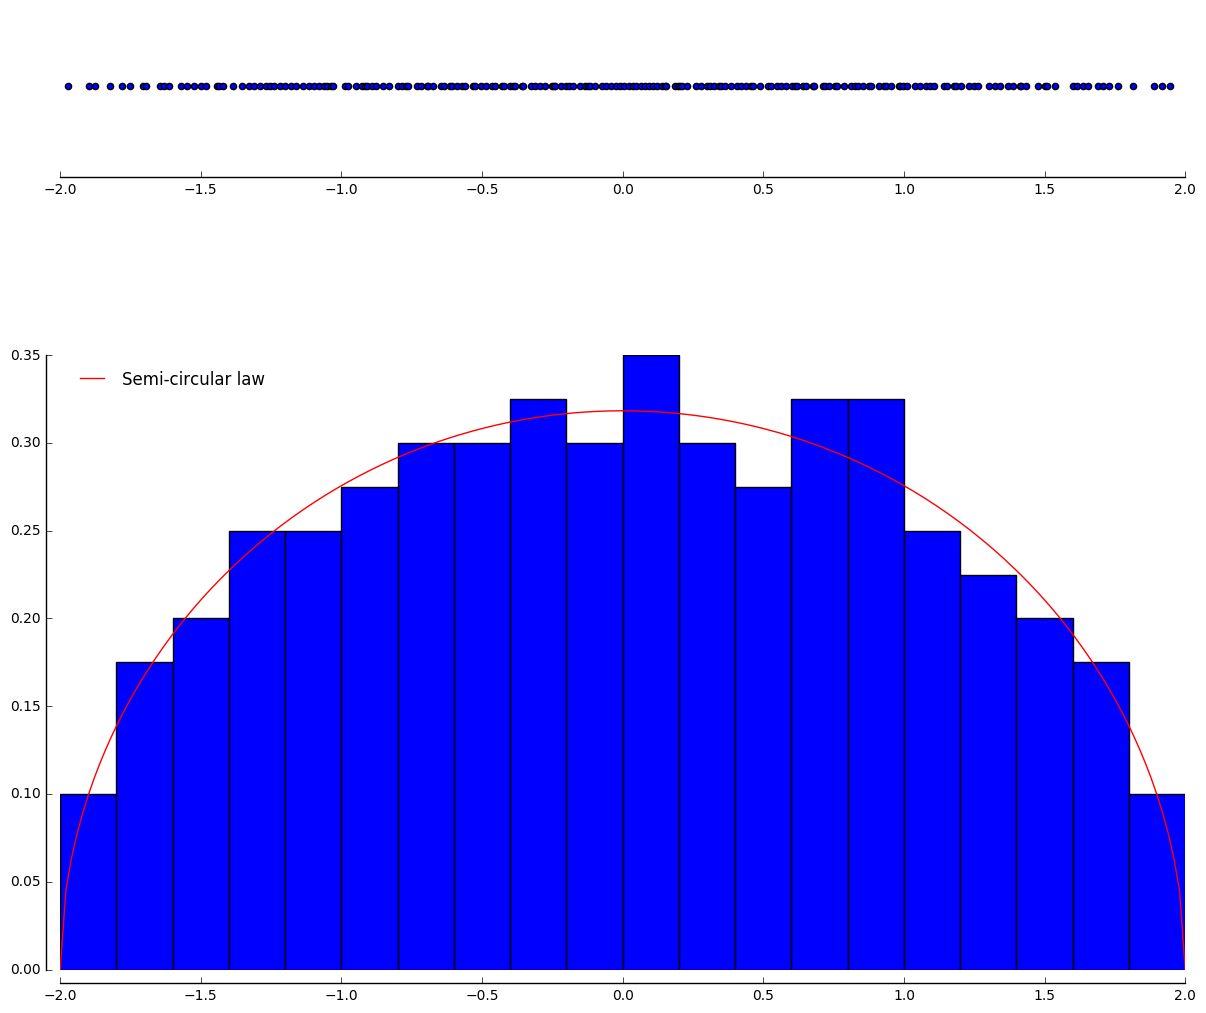
\includegraphics[width=.6\textwidth]{images/tridiag_gue_eigenvalues.png}
				    \caption{\textbf{Eigenvalues histogram of a tridiagonal model for GUE}, generated by the matrix diagonalisation of a $200\times200$ tridiagonal model}\label{fig : tridiag_gue_rescale}
			\end{figure}\ \\ \\
			With Theorem \ref{th : joint distrib trigue}, we can then apply every results from Section \ref{sub:determinantal_point_process}, especially Theorem \ref{th : kernel eig GUE}. Hence, we conclude that the collection of the GUE tridiagonal model eigenvalues is a determinantal point process, with a kernel given by Equation \eqref{eq : kernel GUE}.\\ \\
			To conclude on complexity, if the number of normally distributed random variable generations is the same for a classic GUE and its tridiagonal model, the diagonalisation complexity is reduced from $O(N^3)$ to $O(N^2)$ or even $O(N\ln N)$. It is an significant reduction if we need to simulate a large number of points for a determinantal point process with kernel \eqref{eq : kernel GUE}.
			\begin{remark}[Generalisation of Theorem \ref{th : joint distrib trigue}]\label{rem: generalisation beta ens ??}
				Theorem \ref{th : joint distrib trigue} can be easily apply to GOE and GSE (Gaussian Symplectic Ensemble) using approximately the same proof. However, in \cite{dumitriu2002matrix}, this result is given for even more general ensemble, called the $\beta$-ensembles. In particuler, $\beta$-ensembles gather GOE ($\beta=1$), GUE ($\beta=2$) and GSE ($\beta=4$). The proof is much more complicated for this general case, and cover the majority of the article \cite{dumitriu2002matrix}.\\
				Recall that the whole point of our study is to spread well known static models (e.g. GUE, Wishart). Hence, an open question raised here is to find a dynamic tridiagonal model for the global $\beta$-ensembles.
			\end{remark}
		% subsection tridiagonal_matrice_and_eigenvalues (end)
	% section tridiagonal_model_for_gue_matrices (end)

		\subsection{Naive tridiagonal model for Dyson Brownian motion} % (fold)
		\label{sec:naive_tridiagonal_dyson_brownian_motion}
			The first part of this section gives us intuitions to build a naive dynamic version of the tridiagonal model for GUE matrices. We present it, and its limits before explain the exact solution proposed in \cite{2017arXiv170702700H}.

			The first naive idea is to transform the Definition \ref{def:tridiag mat GUE} into a process over time. To do that, let us first introduce Bessel processes.
			\begin{definition}[Bessel process]\label{def : bessel process}
					The Bessel process of order $k$ is the real-valued process $(S(t))_{t\geq0}$ given by
					\[S(t)=\sqrt{\sum_{i=1}^kB_i(t)^2}=||B(t)||_2\]
					where $||.||_2$ denotes the Euclidean norm in $\mathbb R^k$ and $(\pmb B_i)_{1\leq i\leq k}$ is a $k$-dimensional independent Brownian motion starting at 0.
			\end{definition}
			We make a parallel between the $\chi_k$ distribution and define the naive Brownian and Bessel tridiagonal process.

			\begin{definition}[Naive Brownian and Bessel tridiagonal process]\label{def : naive bb process}
				Let $(\pmb B_i)_{1\leq i\leq N}$ be a collection of i.i.d. real valued standard Brownian motion and $(\pmb S_i)_{1\leq i\leq N}$ be an independent collection of Bessel processes of order $2(N-i)$. Those two collections are also independent. The naive Brownian and Bessel tridiagonal process noted $\pmb T$ is the random process with entries $(\pmb T_{ij})_{1\leq i,j\leq N}$ so that
				\begin{align*}
					\pmb T_{ij}= \left\{
			    					\begin{array}{ll}
			        					\frac{1}{\sqrt{2N}}\ \pmb S_i & \emph{if}\ i=j+1  \\
			        					\frac{1}{\sqrt{N}}\ \pmb B_{i} & \emph{if}\ i=j
			    					\end{array}
								\right.\notag
				\end{align*}
				and completed by symmetry.
			\end{definition}

			We can now consider a random matrix SDE satisfied by a$\ N\times N$ matrix process $\pmb X$, for example : $X_t=A+T_t$ with $A$ a $N\times N$ Hermitian matrix and $\pmb T$ a $N\times N$ Naive Brownian and Bessel tridiagonal process as defined in \ref{def : naive bb process}. This is the same procedure as in Section \ref{sub:Random matrix-valued process}. Thus, we can simulate as explain on Algorithm \ref{alg: tridiag_naive_brownian_bessel} (available on \cite{sebastienGithub}) and get the result shown on Figure \ref{fig : bessel_brownian_tridiag}.

			\begin{algorithm}[H]
						\begin{algorithmic}
						\STATE \textbf{input :} $A,\ N,\ n_{samples},\ t_f$
						\STATE \textbf{initialisation :} 
						\STATE $X \leftarrow 0_{\mathcal{M}_N(\mathbb{R})}$
						\STATE $B_{\chi^2} \leftarrow \{ [0]_{k=1}^{2l}$ \textbf{for} $l=1$ \textbf{to} $N-1\}$
						\STATE $B_{diag} \leftarrow [0]_{k=1}^N$
						\STATE $\Lambda \leftarrow \{OrderedSpectrum(A)\}$
						\STATE $dt\leftarrow t_f/n_{samples}$

						\FOR{t=1 \TO $n_{sample}$}

						\FOR[\textit{fill the diagonal}]{j=1 \textbf{to}$\ N$}
						\STATE draw $G\sim\mathcal{N}(0,1)$
						\STATE $B_{diag}(j)\leftarrow B_{diag}(j) + \sqrt{dt/N}*G$
						\STATE $X(j,j) = B_{diag}(j)$
						\ENDFOR

						\FOR[\textit{fill the upper and lower diagonal}]{j=1 \TO $N-1$}
						\FOR {k=1 \TO $2j$}
						\STATE draw $G\sim{N}(0,1/2)$
						\STATE $B_{\chi^2}(j,k)\leftarrow B_{\chi^2}(j,k) + \sqrt{dt/2N}*G $
						\ENDFOR
						\STATE $X(N-j,N+1-j) = \sqrt{\sum_{k=1}^jB_{\chi^2}(j,k)^2}$
						\STATE $X(N+1-j,N-j) = \sqrt{\sum_{k=1}^jB_{\chi^2}(j,k)^2}$
						\ENDFOR
						\STATE $\Lambda\leftarrow\Lambda\cup\{OrderedSpectrum(X)\}$
						\ENDFOR
						\STATE \textbf{output :} $\Lambda$
						\end{algorithmic}
						\caption{Generation of naive Brownian and Bessel process}
						\label{alg: tridiag_naive_brownian_bessel}
			\end{algorithm}

			This figure is close to the classical Dyson Brownian motion Figure \ref{fig : dyson_brownian_motion}, however, the eigenvalues trajectories seems to be less Brownian in this case, and more smooth. Mathematically, this is because this tridiagonal model does not ensure the eigenvalues to follow the system of SDEs \eqref{eq : dyson-for}. In fact, we only have the following result on the law of the matrix $T_t\sim \sqrt{t}\ T$ when initial condition $A=0_{\mathcal{M}_N(\mathbb{R})}$. Hence, at $t=1$, the eigenvalues of $T_1$ have their joint distribution equals to the GUE eigenvalues joint distribution.\\
			In a nutshell, with this process we manage to obtain the desired joint distribution for the eigenvalues at a particular time, but we do not have the dynamic i.e. the system of SDEs verifyed by the eigenvalues. This remark motivates the following development in the next section.
			\begin{figure}[h] \centering
				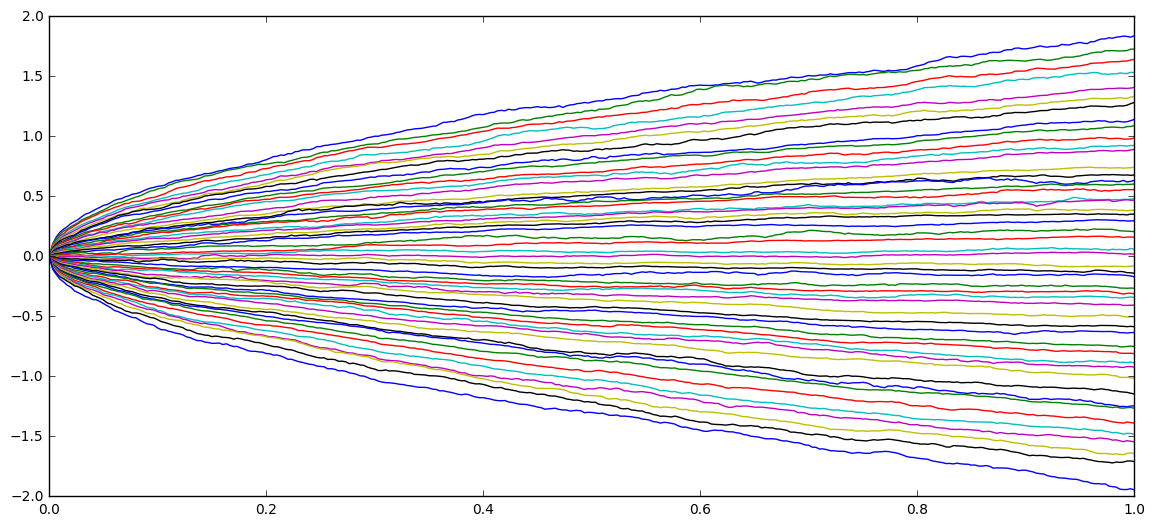
\includegraphics[width=1\textwidth]{images/tridiag_dyn.png}
				\caption{\textbf{Eigenvalues trajectories of a naive Brownian and Bessel tridiagonal model.} 50 eigenvalues, with 300 points in$\ [0,1]$ and initial condition $A=0_{\mathcal{M}_N(\mathbb{R})}$.}\label{fig : bessel_brownian_tridiag}
			\end{figure}

			\begin{remark}[Other tridiagonal process intuition]\label{rem:}
				Another intuition to build a tridiagonal process imitating the Dyson Brownian motion could be to follow the proof of Theorem \ref{th : joint distrib trigue} dynamically. Because the matrix $L$ only depends on $x$, we could build a process $L_t$, depending on entries of a Hermitian Brownian motion. Thus, a tridiagonal process $\pmb T$ (not necessarily as defined in \ref{def : naive bb process}) could be computed from a Hermitian Brownian motion $\pmb H$ so that $\pmb H=\pmb L\pmb T\pmb L^*$.\\
				In practise, the justification is much more complicated than that, and we need to read through \cite{2017arXiv170702700H} to understand the whole mathematical machinery.
			\end{remark}
		% subsection naive_tridiagonal_dyson_brownian_motion (end)

	\section{Exact tridiagonal model for Dyson Brownian motion} % (fold)
	\label{sec:exact_tridiagonal_model_for_dyson_brownian_motion}
		In this part, we aim to give an idea of the process to compute an exact tridiagonal model for the Dyson Brownian motion. The complete mathematical justification is long and rough, but well explained in \cite{2017arXiv170702700H}. Here, we will just try to explain how the principal concepts, on a simulation point of view. The goal is to simulate a matrix-valued random process which preserves the tridiagonal model for GUE. Here, we will never carry out tridiagonalisation, but we will deal with tridiagonal matrices at each time. More precisely, let us denote by $\pmb X$ this tridiagonal process, then $X_t\sim$ TriGUE(N) for $t\geq0$.\\ 
		This operation is complex and rest on the use of discrete orthogonal polynomials defined hereafter. We only develop the desired case of the tridiagonal model for GUE but the reader should know that it was describe for more general models in \cite{2017arXiv170702700H}. In the following development, we try to stay as close as possible to the notation of \cite{2017arXiv170702700H}.

		\begin{remark}[Dynamic tridiagonal model for $\beta$-ensembles]\label{rem:}
			In \cite{2017arXiv170702700H}, authors give an answer to the previous Remark \ref{rem: generalisation beta ens ??}. Indeed, they develop a very general tridiagonal model which covers the $\beta$-ensembles.
		\end{remark}

		\subsection{Discrete orthogonal polynomials} % (fold)
		\label{sub:discrete_orthogonal_polynomials}
			Let $T\sim$ TriGUE(N), we define its coefficient so that  
			\begin{equation}\label{eq : H_beta matrices}
					T = \left( 
						\begin{array}{ccccc}
						b_1  & a_1 &   & & 0\\
				       	a_1 & b_2  & a_2 & & \\
				  			& \ddots   & \ddots    &  \ddots & \\
				         & & a_{N-2} & b_{N-1} &  a_{N-1} \\
				        0 & & & a_{N-1} & b_N
				        \end{array}  \right)\notag
			\end{equation}
			We define a sequence of polynomials $(p_k(x))_{0\leq k\leq N}$ and $\underline p=[p_0(x),p_1(x),\dots,p_{N-1}(x)]$to be the solution of 
			\begin{equation}\label{eq : polynom mat equation}
				T\underline p(x)=x\underline p(x)
			\end{equation}
			Setting $p_0(x)=1$, Equation \eqref{eq : polynom mat equation} describes a three term recurrence
			\begin{align}
				b_1p_0(x)+a_1p_1(x)&=xp_0(x)\notag\\
				a_{k-1}p_{k-2}(x)+b_kp_{k-1}(x)+a_kp_k(x) &= xp_{k-1}(x)\notag\\
				a_{N-1}p_{N-2}(x)+(b_N-x)p_{N-1}(x)&=-p_N(x)\notag
			\end{align}
			Note that if $\lambda$ is an eigenvalue of $T$, then $p_N(\lambda)=0$ and its associate eigenvalue is given by $\underline p(\lambda)$. We now number the eigenvalues like in the previous part, so that $\lambda_1<\lambda_2<\dots<\lambda_N$. \\
			Let $q_i$ be the spectral weight associated to $\lambda_i$ by 
			\begin{equation}
				q_i=\frac{1}{||\underline p(\lambda_i)||_2}\notag
			\end{equation}
			Then, we define the polynomials $p_l^{(k)}(x)$ for any $0\leq k,l\leq N-1$
			\begin{equation}
				p_l^{(k)}(x)=\sum_{j=1}^Nq_j^2p_k(\lambda_j)\frac{p_l(x)-p_l(\lambda_j)}{x-\lambda_j}
			\end{equation}
			for $x$ not in the spectrum. By continuity, we have 
			\begin{equation}
				p_l^{(k)}(\lambda_i)=q_ip_k(\lambda_i)p_k'(\lambda_i)+\sum_{\substack{j=1\\j\neq i}}^Nq_j^2p_k(\lambda_j)\frac{p_l(\lambda_i)-p_l(\lambda_j)}{\lambda_i-\lambda_j}
			\end{equation}
			These polynomials are fundamental in the article \cite{2017arXiv170702700H} to describe the stability of tridiagonal models. In this work, we will only present useful matrices for the simulation of the Dyson Brownian motion tridiagonal model.

		\subsection{Useful matrices for the simulation} % (fold)
		\label{sub:useful_matrices_for_the_simulation}
			First, we need to define the matrix $G(x)$ so that
			\begin{align*}
				G(x)_{kl}= \left\{
			    	\begin{array}{ll}
						a_{l-1}p_{l-2}(x)p_{l-1}(x) - a_lp_{l-1}(x)p_l(x) & \\ 
						+a_{l-1}p_{l-1}(x)p_{l-2}(x)-a_lp_l(x)p_{l-1}(x) & \text{if}\ k=l  \\
	   					a_l(p_{l-1}(x)p_{l-1}(x)-p_l(x)p_l(x)) & \text{if}\ k=l+1 \\
	   					0 & \text{otherwise}		
	   				\end{array}
					\right.\notag
			\end{align*} 
			and completed by symmetry.\\ \\
			Then, we have the matrix $G^{k,l}$ which derive from the matrix $G$ but change on the polynomials coefficients
			\begin{align*}
				G_{ur}^{kl}=\frac{1}{2}\sum_{i=1}^Nq_i^2p_{k-1}(\lambda_i) \left\{
			    	\begin{array}{ll}
						a_{r-1}p_{r-2}(\lambda_i)p_{r-1}^{(l-1)}(\lambda_i) - a_rp_{r-1}(\lambda_i)p_r^{(l-1)}(\lambda_i) & \\ 
						+a_{r-1}p_{r-1}(\lambda_i)p_{r-2}^{(l-1)}(\lambda_i)-a_rp_r(\lambda_i)p_{r-1}^{(l-1)}(\lambda_i) & \text{if}\ u=r<n  \\
	   					a_r(p_{r-1}(\lambda_i)p_{r-1}^{(l-1)}(\lambda_i)-p_r(\lambda_i)p_r^{(l-1)}(\lambda_i)) & \text{if}\ k=l+1 \\
	   					0 & \text{otherwise}		
	   				\end{array}
					\right.\notag
			\end{align*} 
			Note that $G$ and $G^{kl}$ are both tridiagonal symmetric matrices.\\
			With this latter matrix, we can define the sum $\sum_{k\geq l}dP_{k,l,t}\ G^{kl}$. In our case this sum simplify and can be written
			\begin{equation}
				\sum_{k\geq l}dP_{k,l,t}\ G^{kl}=dS_t+dR_t\notag
			\end{equation}
			where $dR_t$ is a lower term, which will be considered negligible for the simulations. Hence, we consider
			\begin{equation}\label{eq : decomposition de sum dP}
				\sum_{k\geq l}dP_{k,l,t}\ G^{kl}\approx dS_t
			\end{equation}
			Still, we have an expression for $dS_t$
			\begin{equation*}
				dS_t = \sum_{i,k,l}^N -\frac{q_i^2}{2}(p_{k-1}(\lambda_i)p_{l-1}'(\lambda_i)+p_{k-1}'(\lambda_i)p_{l-1}(\lambda_i))\ G^{kl}\ dt
			\end{equation*}
			With all of these definitions, we can now present the fundamental theorem that justify the algorithmic simulations.
		% subsection useful_matrices_for_the_simulation (end)
		\newpage
		\subsection{Fundamental theorem and algorithm} % (fold)
		\label{sub:fundamental_theorem_and_algorithm}
			This theorem correponds to the Theorem 18 in \cite{2017arXiv170702700H} and its corollary to Corollary 19.
			We present it in our specific case, the Dyson evolution of the GUE i.e. we set $V(x)=x^2/2$ in Equation \ref{eq : general eig SDE with drift}.
			\begin{theorem}\label{th : HP for frozen weight}
				Let the $q_i$ be fixed then the tridiagonal model associated to the Dyson Brownian motion
				\begin{equation}
					dX_t=\sum_{i=1}^N-\left(dw_{i}(t)+dt\left(\frac{\lambda_{i}(t)}{2}+\sum_{\substack{j=1\\j\neq i}}^N\frac{1}{\lambda_{i}(t)-\lambda_{j}(t)}\right)\right)\ q_i^2\ G(\lambda_{i}(t)) + \sum_{k\geq l}dP_{k,l,t}\ G^{kl}\notag
				\end{equation}
				with with$\ (w_{i}(t))_{1\leq i\leq N}$ a collection of independent real standard Brownian motions driving the Dyson Brownian motion in \ref{eq : general eig SDE with drift}.
				Moreover, denoting by $\pmb \Lambda$ the diagonal process assciated to $\pmb X$ i.e. $\pmb X=\pmb O\pmb \Lambda\pmb O^t$,  if $\pmb \Lambda$ is a stationary process, then $\pmb X$ will be stationary. The definitions of G, $G^{kl}$ and the sum may be found in Section \ref{sub:useful_matrices_for_the_simulation}.
			\end{theorem}
			\begin{corollary}
				If we take $X_0\sim$ \text{TriGUE(N)}, and $\pmb \Lambda$ statisfies the Dyson Brownian flow \ref{eq : general eig SDE with drift} with $V(x)=x^2/2$, then $X_t\sim$ \text{TriGUE(N)} for $t\geq0$.
			\end{corollary}
			This leads us to the following simplyfied Algorithm \ref{alg: holcomb paquette}, the complete version is available on \cite{sebastienGithub}.
			\begin{algorithm}[H]
					\begin{algorithmic}
					\STATE \textbf{input :} $A,\ N,\ n_{samples},\ t_f$
					\STATE \textbf{initialisation :} 
					\STATE $dt\leftarrow t_f/n_{samples}$
					\STATE $\Lambda \leftarrow \{OrderedSpectrum(A)\}$
					\STATE $q\leftarrow SpectralWeights(A)$
					\STATE $X \leftarrow A$
					\FOR{t=1 \textbf{to}$\ n_{sample}$}
					\STATE draw$\ B\sim \mathcal{N}(0,1)$
					\STATE $p\leftarrow Polynomials(X)$
					\STATE $G\leftarrow G(X,p,\Lambda(t))$
					\STATE $dS\leftarrow S(X,p,\Lambda(t),G^{kl})$
					\STATE $dX\leftarrow \sum_{i=1}^N-\left(\sqrt{dt/N}B+dt\left(\frac{\Lambda(t,i)}{2}+\sum_{j\neq i}\frac{1}{\lambda(t,i)-\lambda(t,j)}\right)\right)q(i)^2G + dS$
					\STATE $X \leftarrow X + dX$
					\STATE $\Lambda \leftarrow \Lambda \cup \{OrderedSpectrum(X)\}$
					\ENDFOR
					\STATE \textbf{output :} $\Lambda$
					\end{algorithmic}
					\caption{Eigenvalues trajectories simulation with tridiagonal model}
					\label{alg: holcomb paquette}
			\end{algorithm}

			In practise, Algorithm \ref{alg: holcomb paquette} is not easy to implement. Moreover, it does not give satisfying results because after a few increments, the diagonalisation does not converge. The approximations operated to perform simulation (e.g. Equation \eqref{eq : decomposition de sum dP}) may be a fact that affect the eigenvalues trajectories generations.\\
			Furthermore, the reader might notice the form of the SDE in Theorem \ref{th : HP for frozen weight}: it is not an exact simulation of a process. Recall Table \ref{tab : comparison 1}, the latter simulation is closer to the simulation with a system of eigenvalues SDEs than to the other. Let us present a new comparison table.
			\begin{table}[h]
	   			\centering
				  \begin{tabular}{|l|c|c|c|}
				    \cline{2-4}
				    \multicolumn{1}{c|}{} & Matrix SDE & Tridiagonal SDE& Eigenvalues SDEs \\ \hline
				    Type of simulation & Exact & Approximate & Approximate  \\ \hline
				    $\#$ simulations $\sim\mathcal N$ & $2N^2$ & $N$ & $N$ \\ \hline
				    Diagonalisation & $O(N^3)$   &$O(N^2)$ or $O(N\ln N)$ & None  \\ \hline
				    Robustness & High & Low (for this simulation) & Low ("jumps") \\ \hline 
				  \end{tabular}
				\caption{Comparison of the three simulation methods}\label{tab : comparison 2}	
			\end{table}\ \\
			We observe that the simulation with the tridiagonal model is a good trade-off between the two previous one. However, we cannot really conclude on its performance because we do not have any result to present. Some extra time is necessary to provide a complete overview of this model on a simulation scale. Moreover, note that a lot of polynomials evaluations are performed that need to be added to compute the exact complexity.
		% subsection fundamental_theorem_and_algorithm (end)	

	% section exact_tridiagonal_model_for_dyson_brownian_motion (end)

	
\chapter*{Conclusion}
	\addcontentsline{toc}{chapter}{Conclusion}
	In this study, we manage to understand the particular repulsion phenomenon appearing in the Dyson Brownian motion and in other classical examples. Depending on the considered process, we can link the eigenvalues collection at a fixed time to a determinantal point process. These processes are precisely well-known for their repulsion property and characterised the interaction observed between the eigenvalues trajectories at a fixed time.\\

	A big issue was to think about simulations. Matrix processes and eigenvalues trajectories are defined by stochastic differential equations and it is not obvious to find a way to properly generate these processes. Several methods came up, with their pros and cons. Simulations with a random matrix SDE are computationally costly but exact and very robust. On the contrary, simulations with eigenvalues SDEs using a Euler approximation are less costly but approximate and with low robustness. \\

	An interesting trade-off was proposed in a very recent article, using some triadiagonal matrix-values processes. These processes were studied at the end of the master's thesis.
	Hence, an open question left by this work is to find a usable implementation of them. Indeed, we could get a robust way to generate a spreading determinantal point process repulsion for an affordable computational cost. Furthermore, we might use the total contribution of this new article to study tridiagonal models for general $\beta$-ensembles. This could create a significant variety of processes with specific repulsion to characterise.

%\bibliography{biblio}
%\bibliographystyle{apalike}
\printbibliography[title={References}]
\addcontentsline{toc}{chapter}{References}

\appendix
	\chapter{Hadamard's variation formulas}

		\section{Hadamard's first variation formula}\label{hadamard1}

			\begin{proof}[Proof of Lemma \ref{had1}]
				Let $\pmb A$ be a $N\times N$ Hermitian matrix-valued process with simple spectrum. Suppose that $\pmb A$ is a derivable function of $t$. Denoting by $(\lambda(t))_{t\geq 0}$ an eigenvalue of $\pmb A$ and $u=(u(t))_{t\geq 0}$ an associated eigenvector for $t\geq0$, it is known that $\lambda(t)$ and $u(t)$ are derivable. For notation simplification, we do not write the $t$ index for the eigenvector.\newline \newline
				By differentiating the equations 
					\begin{align*} 	A_tu = \lambda(t) u 	\end{align*}
				We get
					\begin{align*} 	\dot{A_t}u + A_t\dot{u} = \dot{\lambda(t)}u + \lambda(t)\dot{u}	 \end{align*}
				By left-composing with$\ u$
					\begin{align*} 	
						u^*\dot{A_t}u + u^*A_t\dot{u} &= u^*\dot{\lambda}(t)u + u^*\lambda(t)\dot{u} \\
						& = \dot{\lambda}(t)u^*u + \lambda(t) u^*\dot{u} \\
						& = \dot{\lambda}(t) + \lambda(t) u^*\dot{u}
					\end{align*}
				Moreover, remember that $A_t$ is Hermitian:$\ u^*A_t = (A_t^*u)^*= (A_tu)^*=(\lambda(t) u)^*=\lambda(t) u^*$. \newline \newline
				Thus
					\begin{align*}
						\dot{\lambda}(t) &= u^*\dot{A}_tu + u^*A_t\dot{u} - \lambda(t) u^*\dot{u} \\
						&=u^*\dot{A}_tu + u^*A_t\dot{u} - u^*A_t\dot{u}
					\end{align*}
				Thus, we conclude the \textit{Hadarmard first formula} 
					\begin{align*}
						\dot{\lambda}(t) = u^*\dot{A_t}u
					\end{align*}
			\end{proof}



		\section{Hadamard's second variation formula}
			\label{hadamard2}

			\begin{proof}[Proof of Lemma \ref{had2}]
				Let $\pmb A$ be a $N\times N$ Hermitian matrix-valued process with simple spectrum.. Suppose that $\pmb A$ is a twice derivable function of $t$. Denoting by $(\lambda_i(t))_{1\leq i\leq N}$ the eigenvalues of $\pmb A$ and $u_i=(u_i(t))_{1\leq i\leq N}$ their associated eigenvectors for $t\geq0$, it is known that $\lambda(t)$ and $u_i(t)$ are twice derivable. For notation simplification, we do not write the $t$ indew for the eigenvectors. \newline \newline
				By differentiating the equations : 
				\begin{align*} 	
					A_tu_{i} = \lambda_{i}(t)u_{i} 	
				\end{align*}
				We get
				\begin{align*} 	
					\dot{A}_tu_{i} + A_t\dot{u_{i}} = \dot{\lambda_{i}}(t)u_{i} + \lambda_{i}(t)\dot{u_{i}}	 
				\end{align*}
				\newline
				For$\ j\ne i\in\{1...n\}$, by left-composing by $u_j$ we have
				\begin{align} 	
					u_j^*\dot{A}_tu_i + u_j^*A_t\dot{u_i} - u_j^*\dot{\lambda_i}(t)u_i - u_j^*\lambda_i(t)\dot{u_i} &=0 \notag \\
					u_j^*\dot{A}_tu_i + u_j^*A_t\dot{u_i} - \dot{\lambda_i}(t)\underbrace{u_j^*u_i}_{=0} - \lambda_i(t)u_j^*\dot{u_i} &=0 \notag \\
					u_j^*\dot{A}_tu_i + u_j^*A_t\dot{u_i} - \lambda_i(t)u_j^*\dot{u_i} &=0 \notag \\
					u_j^*\dot{A}_tu_i + (A_t^*u_j)^*\dot{u_i} - \lambda_i(t)u_j^*\dot{u_i} &=0 \notag
				\end{align}
				Knowing that$\ A_t$ is an hermitian matrix, which means that$\ A_t^*=A_t$
				\begin{align} 	
					u_j^*\dot{A}_tu_i + (A_tu_j)^*\dot{u_i} - \lambda_i(t)u_j^*\dot{u_i} &=0 \notag \\
					u_j^*\dot{A}_tu_i + (\lambda_j(t)u_j)^*\dot{u_i} - \lambda_i(t)u_j^*\dot{u_i} &=0 \notag \\
					u_j^*\dot{A}_tu_i + \lambda_j(t)u_j^*\dot{u_i} - \lambda_i(t)u_j^*\dot{u_i} &=0 \notag \\
					u_j^*\dot{A}_tu_i + (\lambda_j(t)-\lambda_i(t))u_j^*\dot{u_i} &=0 \notag
				\end{align}
				Leading to
				\begin{align} \label{eq:1}
					u_j^*\dot{u_i} = \frac{u_j^*\dot{A}_tu_i}{\lambda_i(t)-\lambda_j(t)}
				\end{align}

				The eigenvectors$\ (u_i)_{i\in\{1...n\}}$ form a basis of$\ \mathbb{C}^n$. Let$\ (v_i)_{i\in\{1...n\}}$ be the dual basis, thus$\ v_j^*u_k=\delta_{jk}$ for all$\ (i,j)\in\{1...n\}^2$. We have the reproducing formula
				\begin{align} \label{eq:2}
					\dot{u_i} &= \sum_{j=1}^n (v_j^*\dot{u_i})u_j
				\end{align}
				$\ A$ is self-adjoint because we suppose that$\ A$ is an hermitian matrix. So we can take the eigenvectors$\ (u_i)_{i\in\{1...n\}}$ to be orthonormal, in which case$\ (v_i)_{i\in\{1...n\}}$ is identical to$\ (u_i)_{i\in\{1...n\}}$.
				\newline \newline
				Equation \eqref{eq:2} becomes
				\begin{align} \label{eq:3}
					\dot{u_i} &= \sum_{j=1}^n (u_j^*\dot{u_i})u_j \notag \\
					\dot{u_i} &= \sum_{\substack{j=1 \\ j \neq i}}^n u_j^*\dot{u_i}u_j + u_i^*\dot{u_i}u_i
				\end{align}
				We introduce \eqref{eq:1} in \eqref{eq:3}
				\begin{align} \label{eq:4}
					\dot{u_i} &= \sum_{\substack{j=1 \\ j \neq i}}^n \frac{u_j^*\dot{A}_tu_i}{\lambda_i(t)-\lambda_j(t)}u_j + u_i^*\dot{u_i}u_i
				\end{align}
				Doing the same with$\ \dot{u_k}^*$ 
				\begin{align} \label{eq:5}
					\dot{u_{i}}^* &= \sum_{j=1}^n (\dot{u_i}^*u_j)u_j^* \notag \\
					\dot{u_{i}}^* &= \sum_{\substack{j=1 \\ j \neq i}}^n \dot{u_i}^*u_ju_j^* + \dot{u_i}^*u_iu_i^* \notag \\
					\dot{u_{i}}^* &= \sum_{\substack{j=1 \\ j \neq i}}^n \frac{u_i^*\dot{A}_tu_j}{\lambda_i(t)-\lambda_j(t)}u_j^* + \dot{u_i}^*u_iu_i^*
				\end{align}
				\newline
				By derivating the \textit{Hadamard first variation formula}$\ (\dot{\lambda_i}=u_i^*\dot{A}u_i)$ and using \eqref{eq:4} and \eqref{eq:5}
				\begin{align} \label{eq:6}
					\ddot{\lambda_i}(t) &= u_i^*\ddot{A}_tu_i + \dot{u_i}^*\dot{A}_tu_i + u_i^*\dot{A}_t\dot{u_i} \notag \\
					\ddot{\lambda_i}(t) &= u_i^*\ddot{A}_tu_i + \Big(\sum_{\substack{j=1 \\ j \neq i}}^n \frac{u_i^*\dot{A}_tu_j}{\lambda_i(t)-\lambda_j(t)}u_j^* + \dot{u_i}^*u_iu_i^*\Big)\dot{A}_tu_i + u_i^*\dot{A}_t\Big(\sum_{\substack{j=1 \\ j \neq i}}^n \frac{u_j^*\dot{A}_tu_i}{\lambda_i(t)-\lambda_j(t)}u_j + u_i^*\dot{u_i}u_i\Big) \notag \\
					\ddot{\lambda_i}(t) &= u_i^*\ddot{A}_tu_i + 2\sum_{\substack{j=1 \\ j \neq i}}^n \frac{(u_i^*\dot{A}_tu_j)(u_j^*\dot{A}_tu_i)}{\lambda_i(t)-\lambda_j(t)} + \dot{u_i}^*u_iu_i^*\dot{A}_tu_i + u_i^*\dot{A}_tu_i^*\dot{u_i}u_i \notag \\
					\ddot{\lambda_i}(t) &= u_i^*\ddot{A}_tu_i + 2\sum_{\substack{j=1 \\ j \neq i}}^n \frac{|u_j^*\dot{A}_tu_i|^2}{\lambda_i(t)-\lambda_j(t)} + \dot{u_i}^*u_iu_i^*\dot{A}_tu_i + u_i^*\dot{u_i}u_i^*\dot{A}_tu_i \notag \\
					\ddot{\lambda_i}(t) &= u_i^*\ddot{A}_tu_i + 2\sum_{\substack{j=1 \\ j \neq i}}^n \frac{|u_j^*\dot{A}_tu_i|^2}{\lambda_i(t)-\lambda_j(t)} + (\dot{u_i}^*u_i + u_i^*\dot{u_i})u_i^*\dot{A}_tu_i
				\end{align}

				By derivating $\ u_{i}^*u_{i} = 1$ we have 
				\begin{align} \label{eq:7}
					\dot{u_{i}}^*u_{i} + u_{i}^*\dot{u_{i}} = 0	
				\end{align}
				\newline \newline
				Applying \eqref{eq:7} in \eqref{eq:6}, we conclude the \textit{Hadamard second variation formula}
				\begin{align*}
					\ddot{\lambda_i} =u_i^*\ddot{A}_tu_i + 2\sum_{\substack{j=1 \\ j \neq i}}^{n} \frac{| u_{j}^*\dot{A}_tu_i |^2}{\lambda_i(t)-\lambda_j(t)}
				\end{align*}
			\end{proof}


	\chapter{Quadratic variations}

		\section{It\^{o} development of Stratonovich integral}\label{dev-strat-pro}

			\begin{proof}[Proof of Lemma \ref{dev-strat}] Let $\pmb X$, $\pmb Y$ and $\pmb Z$ be three It\^{o} processes such that :
			\begin{align}
				& X_t = \int_0^tH_s^XdB_s + \int_0^tK_s^Xds \notag \\
				& Y_t = \int_0^tH_s^YdB_s + \int_0^tK_s^Yds \notag \\
				& Z_t = \int_0^tH_s^ZdB_s + \int_0^tK_s^Zds \notag 
			\end{align}
			We have:
			\begin{align}
					Y_t\circ dX_t\circ Z_t &=  (Y_t\circ dX_t)\circ Z \notag\\
					&=(Y_t^*dX_t +\frac{1}{2}d\langle_t Y,X\rangle) \circ Z_t \notag\\	
					&= (Y_tdX_t +\frac{1}{2}d\langle Y,X\rangle_t)Z_t + V_F \notag \\
					&= Y_tdX_tZ_t +\frac{1}{2}d\langle Y,X\rangle_tZ_t + V_F \notag
			\end{align}
			When we distribute the Stratonovich integral, we will obtain a first term:$\ (Y_tdX_t +\frac{1}{2}d\langle Y,X\rangle_t)Z_t$ and a second term with quadratic variation. \newline
			The second term$\ V_F$ is compute by two terms:$\ Y_tdX_t$ and$\ \frac{1}{2}d\langle Y,X\rangle_t$. But$\ \frac{1}{2}d\langle Y,X\rangle_t$ will not have an impact when we calculate$\ V_F$ because it is a finite variation term itself. \newline
			Let's focus on the term$\ Y_tdX_t$:
			\begin{align}
				\int_0^tY_sdX_s = \int_0^tY_sK_s^Xds+\int_0^tY_sH_s^XdB_s\notag
			\end{align}
			So, we have:
			\begin{align}
				VF &= \frac{1}{2}Y_tH_t^XH_t^Zdt\notag \\
				&=\frac{1}{2}Y_td\langle X,Z\rangle_t \notag
			\end{align}
			Finally, we obtain \eqref{eq : dev strat pro eq}.
			\end{proof}


		\section{Hermitian matrices verifying a general SDE}\label{quad_va2}

			\begin{proof}[Proof of Lemma \ref{quadra_va2}] In order to compute the quadratic variation of the entries, we note
			\begin{align}
					dX_{ij,t} &= (g(X_t)dB_th(X_t) + h(X_t)dB_t^*g(X_t) +b(X_t)dt)_{ij} \notag\\
					&= (g(X_t)dB_th(X_t))_{ij} + (h(X_t)dB_t^*g(X_t))_{ij} +(b(X_t)dt)_{ij} \notag
			\end{align}
			and
			\begin{align}
					dX_{i'j',t} &= (g(X_t)dB_th(X_t) + h(X_t)dB_t^*g(X_t) +b(X_t)dt)_{i'j'} \notag\\
					&= (g(X_t)dB_th(X_t))_{i'j'} + (h(X_t)dB_t^*g(X_t))_{i'j'} +(b(X_t)dt)_{i'j'} \notag
			\end{align}
			When we distribute the quadratic variation, we obtain nine terms. However, terms with$\ b(X_t)dt$ will give a quadratic variation equals to zero. So we will have only four terms in finally.\newline
			\paragraph{Term 1} 
			\begin{align}
				& d\langle (g(X)Bh(X))_{ij}, (g(X)Bh(X))_{i'j'}\rangle_t \notag \\
				&= d\langle \sum_{k,l}g(X)_{ik}B_{kl}h(X)_{lj}, \sum_{m,n}g(X)_{i'm}B_{mn}h(X_t)_{nj'}\rangle_t \notag
			\end{align}
			Using Lemma \ref{quadra_va1}, we know that$\ d\langle B_{kl},B_{mn}\rangle_t \neq0$ if$\ B_{kl}$ and$\ B_{mn}$ are conjuguate. We cannot find$\ m,\ n,\ k$ and$\ l$ to make$\ B_{kl}$ and$\ B_{mn}$ each other conjuguate because $\pmb B$ is a matrix of independant complex Brownian motions. Finally, term 1 is zero.

			\paragraph{Term 2} 
			\begin{align}
				& d\langle (g(X)Bh(X))_{ij}, (g(X)B^*h(X))_{i'j'}\rangle_t \notag\\
				&= d\langle \sum_{k,l}g(X)_{ik}B_{kl}h(X)_{lj}, \sum_{m,n}g(X)_{i'm}B_{mn}^*h(X)_{nj'}\rangle_t \notag \\
				&= d\langle \sum_{k,l}g(X)_{ik}B_{kl}h(X)_{lj}, \sum_{m,n}g(X)_{i'm}\overline{B_{nm}}h(X)_{nj'}\rangle_t \notag
			\end{align}
			Using Lemma \ref{quadra_va1},$\ \langle B_{kl},\overline{B_{nm}}\rangle =2dt$ if$\ k=n$ and$\ l=m$. \newline We have
			\begin{align}
				& d\langle (g(X)Bh(X))_{ij}, (g(X)B^*h(X))_{i'j'}\rangle_t \notag\\
				&= (2dt)\sum_{k,l}g(X)_{ik}h(X)_{lj}h(X)_{i'l}g(X)_{kj'} \notag \\
				&= (2dt)\sum_{k}g(X)_{ik}g(X)_{kj'}\sum_{l}h(X)_{i'l}h(X)_{lj}\notag \\
				&=2(g^2(X))_{ij'}(h^2(X))_{i'j}dt
			\end{align}

			\paragraph{Term 3} 
			\begin{align}
				& d\langle (h(X)B^*g(X))_{ij}, (g(X)dBh(X))_{i'j'}\rangle_t \notag\\
				&= d\langle \sum_{k,l}h(X)_{ik}B_{kl}^*g(X)_{lj}, \sum_{m,n}g(X)_{i'm}B_{mn}h(X)_{jj'}\rangle_t \notag \\
				&= d\langle \sum_{k,l}h(X)_{ik}\overline{B_{lk}}g(X)_{lj}, \sum_{m,n}g(X)_{s'i}B_{nm}h(X)_{nj'}\rangle_t \notag
			\end{align}
			Using \ref{quadra_va1},$\ d\langle B_{kl},\overline{B_{nm}}\rangle =2dt$ if$\ l=m$ and$\ k=n$. \newline We have
			\begin{align}
				& d\langle (h(X)B^*g(X))_{ij}, (g(X)Bh(X))_{i'j'}\rangle_t \notag\\
				&= (2dt)\sum_{k,l}h(X)_{ik}g(X)_{lj}g(X)_{i'l}h(X)_{kj'} \notag \\
				&= (2dt)\sum_{k}h(X)_{ik}h(X)_{kj'}\sum_{l}g(X)_{i'l}g(X)_{lj}\notag \\
				&=2(g^2(X))_{i'j}(h^2(X))_{ij} dt
			\end{align}

			\paragraph{Term 4} 
			\begin{align}
				& d\langle (h(X)B^*g(X))_{ij}, (h(X)B^*g(X))_{i'j'}\rangle_t \notag \\
				&= d\langle \sum_{k,l}h(X)_{ik}B_{kl}^*g(X)_{lj}, \sum_{m,n}h(X)_{i'm}B_{mn}^*g(X)_{nj'}\rangle_t \notag \\
				&= d\langle \sum_{k,l}h(X)_{ik}\overline{B_{lk}}g(X)_{lj}, \sum_{m,n}h(X)_{i'm}\overline{B_{nm}}g(X)_{nj'}\rangle_t \notag
			\end{align}
			For the same reason as term 1, term 4 equals to zero.
			\newline \newline
			Finally, we obtain Equation \eqref{eq : trux bizarre}.
			\end{proof}


\end{document}


